\documentclass[]{article}
\usepackage{lmodern}
\usepackage{amssymb,amsmath}
\usepackage{ifxetex,ifluatex}
\usepackage{fixltx2e} % provides \textsubscript
\ifnum 0\ifxetex 1\fi\ifluatex 1\fi=0 % if pdftex
  \usepackage[T1]{fontenc}
  \usepackage[utf8]{inputenc}
\else % if luatex or xelatex
  \ifxetex
    \usepackage{mathspec}
  \else
    \usepackage{fontspec}
  \fi
  \defaultfontfeatures{Ligatures=TeX,Scale=MatchLowercase}
\fi
% use upquote if available, for straight quotes in verbatim environments
\IfFileExists{upquote.sty}{\usepackage{upquote}}{}
% use microtype if available
\IfFileExists{microtype.sty}{%
\usepackage{microtype}
\UseMicrotypeSet[protrusion]{basicmath} % disable protrusion for tt fonts
}{}
\usepackage[margin=1in]{geometry}
\usepackage{hyperref}
\hypersetup{unicode=true,
            pdftitle={Predictr Code},
            pdfauthor={Kiernan Nicholls},
            pdfborder={0 0 0},
            breaklinks=true}
\urlstyle{same}  % don't use monospace font for urls
\usepackage{color}
\usepackage{fancyvrb}
\newcommand{\VerbBar}{|}
\newcommand{\VERB}{\Verb[commandchars=\\\{\}]}
\DefineVerbatimEnvironment{Highlighting}{Verbatim}{commandchars=\\\{\}}
% Add ',fontsize=\small' for more characters per line
\usepackage{framed}
\definecolor{shadecolor}{RGB}{248,248,248}
\newenvironment{Shaded}{\begin{snugshade}}{\end{snugshade}}
\newcommand{\AlertTok}[1]{\textcolor[rgb]{0.94,0.16,0.16}{#1}}
\newcommand{\AnnotationTok}[1]{\textcolor[rgb]{0.56,0.35,0.01}{\textbf{\textit{#1}}}}
\newcommand{\AttributeTok}[1]{\textcolor[rgb]{0.77,0.63,0.00}{#1}}
\newcommand{\BaseNTok}[1]{\textcolor[rgb]{0.00,0.00,0.81}{#1}}
\newcommand{\BuiltInTok}[1]{#1}
\newcommand{\CharTok}[1]{\textcolor[rgb]{0.31,0.60,0.02}{#1}}
\newcommand{\CommentTok}[1]{\textcolor[rgb]{0.56,0.35,0.01}{\textit{#1}}}
\newcommand{\CommentVarTok}[1]{\textcolor[rgb]{0.56,0.35,0.01}{\textbf{\textit{#1}}}}
\newcommand{\ConstantTok}[1]{\textcolor[rgb]{0.00,0.00,0.00}{#1}}
\newcommand{\ControlFlowTok}[1]{\textcolor[rgb]{0.13,0.29,0.53}{\textbf{#1}}}
\newcommand{\DataTypeTok}[1]{\textcolor[rgb]{0.13,0.29,0.53}{#1}}
\newcommand{\DecValTok}[1]{\textcolor[rgb]{0.00,0.00,0.81}{#1}}
\newcommand{\DocumentationTok}[1]{\textcolor[rgb]{0.56,0.35,0.01}{\textbf{\textit{#1}}}}
\newcommand{\ErrorTok}[1]{\textcolor[rgb]{0.64,0.00,0.00}{\textbf{#1}}}
\newcommand{\ExtensionTok}[1]{#1}
\newcommand{\FloatTok}[1]{\textcolor[rgb]{0.00,0.00,0.81}{#1}}
\newcommand{\FunctionTok}[1]{\textcolor[rgb]{0.00,0.00,0.00}{#1}}
\newcommand{\ImportTok}[1]{#1}
\newcommand{\InformationTok}[1]{\textcolor[rgb]{0.56,0.35,0.01}{\textbf{\textit{#1}}}}
\newcommand{\KeywordTok}[1]{\textcolor[rgb]{0.13,0.29,0.53}{\textbf{#1}}}
\newcommand{\NormalTok}[1]{#1}
\newcommand{\OperatorTok}[1]{\textcolor[rgb]{0.81,0.36,0.00}{\textbf{#1}}}
\newcommand{\OtherTok}[1]{\textcolor[rgb]{0.56,0.35,0.01}{#1}}
\newcommand{\PreprocessorTok}[1]{\textcolor[rgb]{0.56,0.35,0.01}{\textit{#1}}}
\newcommand{\RegionMarkerTok}[1]{#1}
\newcommand{\SpecialCharTok}[1]{\textcolor[rgb]{0.00,0.00,0.00}{#1}}
\newcommand{\SpecialStringTok}[1]{\textcolor[rgb]{0.31,0.60,0.02}{#1}}
\newcommand{\StringTok}[1]{\textcolor[rgb]{0.31,0.60,0.02}{#1}}
\newcommand{\VariableTok}[1]{\textcolor[rgb]{0.00,0.00,0.00}{#1}}
\newcommand{\VerbatimStringTok}[1]{\textcolor[rgb]{0.31,0.60,0.02}{#1}}
\newcommand{\WarningTok}[1]{\textcolor[rgb]{0.56,0.35,0.01}{\textbf{\textit{#1}}}}
\usepackage{graphicx,grffile}
\makeatletter
\def\maxwidth{\ifdim\Gin@nat@width>\linewidth\linewidth\else\Gin@nat@width\fi}
\def\maxheight{\ifdim\Gin@nat@height>\textheight\textheight\else\Gin@nat@height\fi}
\makeatother
% Scale images if necessary, so that they will not overflow the page
% margins by default, and it is still possible to overwrite the defaults
% using explicit options in \includegraphics[width, height, ...]{}
\setkeys{Gin}{width=\maxwidth,height=\maxheight,keepaspectratio}
\IfFileExists{parskip.sty}{%
\usepackage{parskip}
}{% else
\setlength{\parindent}{0pt}
\setlength{\parskip}{6pt plus 2pt minus 1pt}
}
\setlength{\emergencystretch}{3em}  % prevent overfull lines
\providecommand{\tightlist}{%
  \setlength{\itemsep}{0pt}\setlength{\parskip}{0pt}}
\setcounter{secnumdepth}{0}
% Redefines (sub)paragraphs to behave more like sections
\ifx\paragraph\undefined\else
\let\oldparagraph\paragraph
\renewcommand{\paragraph}[1]{\oldparagraph{#1}\mbox{}}
\fi
\ifx\subparagraph\undefined\else
\let\oldsubparagraph\subparagraph
\renewcommand{\subparagraph}[1]{\oldsubparagraph{#1}\mbox{}}
\fi

%%% Use protect on footnotes to avoid problems with footnotes in titles
\let\rmarkdownfootnote\footnote%
\def\footnote{\protect\rmarkdownfootnote}

%%% Change title format to be more compact
\usepackage{titling}

% Create subtitle command for use in maketitle
\newcommand{\subtitle}[1]{
  \posttitle{
    \begin{center}\large#1\end{center}
    }
}

\setlength{\droptitle}{-2em}

  \title{Predictr Code}
    \pretitle{\vspace{\droptitle}\centering\huge}
  \posttitle{\par}
    \author{Kiernan Nicholls}
    \preauthor{\centering\large\emph}
  \postauthor{\par}
      \predate{\centering\large\emph}
  \postdate{\par}
    \date{Spring, 2019}


\begin{document}
\maketitle

\begin{Shaded}
\begin{Highlighting}[]
\CommentTok{# devtools::install_github("hrbrmstr/wayback")}
\CommentTok{# utils::install.packages("tidyverse)}
\KeywordTok{library}\NormalTok{(wayback)}
\KeywordTok{library}\NormalTok{(tidyverse)}
\end{Highlighting}
\end{Shaded}

\begin{verbatim}
## -- Attaching packages --------------------------------------------------- tidyverse 1.2.1 --
\end{verbatim}

\begin{verbatim}
## v ggplot2 3.1.1       v purrr   0.3.2  
## v tibble  2.1.1       v dplyr   0.8.0.1
## v tidyr   0.8.3       v stringr 1.4.0  
## v readr   1.3.1       v forcats 0.4.0
\end{verbatim}

\begin{verbatim}
## -- Conflicts ------------------------------------------------------ tidyverse_conflicts() --
## x dplyr::filter() masks stats::filter()
## x dplyr::lag()    masks stats::lag()
\end{verbatim}

\hypertarget{read-archived-input-data}{%
\subsection{Read Archived Input Data}\label{read-archived-input-data}}

\begin{Shaded}
\begin{Highlighting}[]
\NormalTok{DailyMarketData <-}
\StringTok{  }\NormalTok{here}\OperatorTok{::}\KeywordTok{here}\NormalTok{(}\StringTok{"data"}\NormalTok{, }\StringTok{"DailyMarketData.csv"}\NormalTok{) }\OperatorTok
\StringTok{  }\KeywordTok{read_delim}\NormalTok{(}\DataTypeTok{delim =} \StringTok{"|"}\NormalTok{,}
             \DataTypeTok{na =} \StringTok{"n/a"}\NormalTok{,}
             \DataTypeTok{col_types =} \KeywordTok{cols}\NormalTok{(}
               \DataTypeTok{MarketId =} \KeywordTok{col_character}\NormalTok{(),}
               \DataTypeTok{ContractName =} \KeywordTok{col_character}\NormalTok{(),}
               \DataTypeTok{ContractSymbol =} \KeywordTok{col_character}\NormalTok{(),}
               \DataTypeTok{Date =} \KeywordTok{col_date}\NormalTok{(}\DataTypeTok{format =} \StringTok{""}\NormalTok{)))}

\NormalTok{Market_ME02 <-}
\StringTok{  }\NormalTok{here}\OperatorTok{::}\KeywordTok{here}\NormalTok{(}\StringTok{"data"}\NormalTok{, }\StringTok{"Market_ME02.csv"}\NormalTok{) }\OperatorTok
\StringTok{  }\KeywordTok{read_csv}\NormalTok{(}\DataTypeTok{col_types =} \KeywordTok{cols}\NormalTok{(}\DataTypeTok{ContractID =} \KeywordTok{col_character}\NormalTok{(),}
                            \DataTypeTok{Date =} \KeywordTok{col_date}\NormalTok{(}\DataTypeTok{format =} \StringTok{"%m/%d/%Y"}\NormalTok{)))}

\NormalTok{Contract_NY27 <-}
\StringTok{  }\NormalTok{here}\OperatorTok{::}\KeywordTok{here}\NormalTok{(}\StringTok{"data"}\NormalTok{ , }\StringTok{"Contract_NY27.csv"}\NormalTok{) }\OperatorTok
\StringTok{  }\KeywordTok{read_csv}\NormalTok{(}\DataTypeTok{na =} \KeywordTok{c}\NormalTok{(}\StringTok{"n/a"}\NormalTok{, }\StringTok{"NA"}\NormalTok{),}
           \DataTypeTok{skip =} \DecValTok{156}\NormalTok{, }\CommentTok{# this file was a mess}
           \DataTypeTok{col_types =} \KeywordTok{cols}\NormalTok{(}\DataTypeTok{ContractID =} \KeywordTok{col_character}\NormalTok{(),}
                            \DataTypeTok{Date =} \KeywordTok{col_date}\NormalTok{(}\DataTypeTok{format =} \StringTok{"%m/%d/%Y"}\NormalTok{)))}
\end{Highlighting}
\end{Shaded}

\begin{Shaded}
\begin{Highlighting}[]
\CommentTok{## Current members of the 115th}
\CommentTok{## Archived: 2018-10-22 at 18:11}
\NormalTok{legislators_current <-}
\StringTok{  "https://theunitedstates.io/congress-legislators/legislators-current.csv"} \OperatorTok
\StringTok{  }\KeywordTok{read_memento}\NormalTok{(}\DataTypeTok{timestamp =} \StringTok{"2018-10-22"}\NormalTok{, }\DataTypeTok{as =} \StringTok{"raw"}\NormalTok{) }\OperatorTok
\StringTok{  }\KeywordTok{read_csv}\NormalTok{(}\DataTypeTok{col_types =} \KeywordTok{cols}\NormalTok{(}\DataTypeTok{govtrack_id =} \KeywordTok{col_character}\NormalTok{()))}

\CommentTok{# The ideology and leadership scores of the 115th}
\CommentTok{# Calculated with cosponsorship analysis}
\CommentTok{# Archived 2019-01-21 17:13:08}
\NormalTok{sponsorshipanalysis_h <-}
\StringTok{  }\KeywordTok{str_c}\NormalTok{(}\StringTok{"https://www.govtrack.us/"}\NormalTok{,}
        \StringTok{"data/analysis/by-congress/115/sponsorshipanalysis_h.txt"}\NormalTok{) }\OperatorTok
\StringTok{  }\KeywordTok{read_memento}\NormalTok{(}\DataTypeTok{timestamp =} \StringTok{"2019-03-23"}\NormalTok{, }\DataTypeTok{as =} \StringTok{"raw"}\NormalTok{) }\OperatorTok
\StringTok{  }\KeywordTok{read_csv}\NormalTok{(}\DataTypeTok{col_types =} \KeywordTok{cols}\NormalTok{(}\DataTypeTok{ID =} \KeywordTok{col_character}\NormalTok{()))}

\NormalTok{sponsorshipanalysis_s <-}
\StringTok{  }\KeywordTok{str_c}\NormalTok{(}\StringTok{"https://www.govtrack.us/"}\NormalTok{,}
        \StringTok{"data/analysis/by-congress/115/sponsorshipanalysis_s.txt"}\NormalTok{) }\OperatorTok
\StringTok{  }\KeywordTok{read_memento}\NormalTok{(}\DataTypeTok{timestamp =} \StringTok{"2019-03-23"}\NormalTok{, }\DataTypeTok{as =} \StringTok{"raw"}\NormalTok{) }\OperatorTok
\StringTok{  }\KeywordTok{read_csv}\NormalTok{(}\DataTypeTok{col_types =} \KeywordTok{cols}\NormalTok{(}\DataTypeTok{ID =} \KeywordTok{col_character}\NormalTok{()))}
\end{Highlighting}
\end{Shaded}

\begin{Shaded}
\begin{Highlighting}[]
\CommentTok{## District level 538 House model history}
\CommentTok{## Updated:  2018-11-06 at 01:56}
\CommentTok{## Archived: 2018-11-06 at 12:06}
\NormalTok{house_district_forecast <-}
\StringTok{  }\KeywordTok{str_c}\NormalTok{(}\DataTypeTok{site =} \StringTok{"https://projects.fivethirtyeight.com/"}\NormalTok{,}
        \DataTypeTok{file =} \StringTok{"congress-model-2018/house_district_forecast.csv"}\NormalTok{) }\OperatorTok
\StringTok{  }\KeywordTok{read_memento}\NormalTok{(}\DataTypeTok{timestamp =} \StringTok{"2018-11-06"}\NormalTok{, }\DataTypeTok{as =} \StringTok{"raw"}\NormalTok{) }\OperatorTok
\StringTok{  }\KeywordTok{read_csv}\NormalTok{()}
\end{Highlighting}
\end{Shaded}

\begin{verbatim}
## Parsed with column specification:
## cols(
##   forecastdate = col_date(format = ""),
##   state = col_character(),
##   district = col_double(),
##   special = col_logical(),
##   candidate = col_character(),
##   party = col_character(),
##   incumbent = col_logical(),
##   model = col_character(),
##   win_probability = col_double(),
##   voteshare = col_double(),
##   p10_voteshare = col_double(),
##   p90_voteshare = col_double()
## )
\end{verbatim}

\begin{Shaded}
\begin{Highlighting}[]
\CommentTok{# Seat level 538 Senate model history}
\CommentTok{# Updated:  2018-11-06 at 11:06}
\CommentTok{# Archived: 2018-11-06 at 21:00}
\NormalTok{senate_seat_forecast <-}
\StringTok{  }\KeywordTok{str_c}\NormalTok{(}\DataTypeTok{site =} \StringTok{"https://projects.fivethirtyeight.com/"}\NormalTok{,}
        \DataTypeTok{file =} \StringTok{"congress-model-2018/senate_seat_forecast.csv"}\NormalTok{) }\OperatorTok
\StringTok{  }\KeywordTok{read_memento}\NormalTok{(}\DataTypeTok{timestamp =} \StringTok{"2018-11-06"}\NormalTok{, }\DataTypeTok{as =} \StringTok{"raw"}\NormalTok{) }\OperatorTok
\StringTok{  }\KeywordTok{read_csv}\NormalTok{()}
\end{Highlighting}
\end{Shaded}

\begin{verbatim}
## Parsed with column specification:
## cols(
##   forecastdate = col_date(format = ""),
##   state = col_character(),
##   class = col_double(),
##   special = col_logical(),
##   candidate = col_character(),
##   party = col_character(),
##   incumbent = col_logical(),
##   model = col_character(),
##   win_probability = col_double(),
##   voteshare = col_double(),
##   p10_voteshare = col_double(),
##   p90_voteshare = col_double()
## )
\end{verbatim}

\begin{Shaded}
\begin{Highlighting}[]
\CommentTok{# Midterm election results via ABC and 538}
\CommentTok{# Used in https://53eig.ht/2PiFb0f}
\CommentTok{# Published: 2018-12-04 at 17:56}
\CommentTok{# Archived:  2018-04-04 at 16:08}
\NormalTok{forecast_results_}\DecValTok{2018}\NormalTok{ <-}
\StringTok{  }\KeywordTok{str_c}\NormalTok{(}\DataTypeTok{site =} \StringTok{"https://raw.githubusercontent.com/"}\NormalTok{,}
        \DataTypeTok{fold =} \StringTok{"fivethirtyeight/data/master/forecast-review/"}\NormalTok{,}
        \DataTypeTok{file =} \StringTok{"forecast_results_2018.csv"}\NormalTok{) }\OperatorTok
\StringTok{  }\KeywordTok{read_memento}\NormalTok{(}\DataTypeTok{timestamp =} \StringTok{"2019-04-04"}\NormalTok{, }\DataTypeTok{as =} \StringTok{"raw"}\NormalTok{) }\OperatorTok
\StringTok{  }\KeywordTok{read_csv}\NormalTok{(}\DataTypeTok{col_types  =} \KeywordTok{cols}\NormalTok{(}
    \DataTypeTok{Democrat_Won =} \KeywordTok{col_logical}\NormalTok{(),}
    \DataTypeTok{Republican_Won =} \KeywordTok{col_logical}\NormalTok{(),}
    \DataTypeTok{uncalled =} \KeywordTok{col_logical}\NormalTok{(),}
    \DataTypeTok{forecastdate =} \KeywordTok{col_date}\NormalTok{(}\DataTypeTok{format =} \StringTok{"%m/%d/%y"}\NormalTok{),}
    \DataTypeTok{category =} \KeywordTok{col_factor}\NormalTok{(}\DataTypeTok{ordered =} \OtherTok{TRUE}\NormalTok{,}
                          \DataTypeTok{levels =} \KeywordTok{c}\NormalTok{(}\StringTok{"Solid D"}\NormalTok{,}
                                     \StringTok{"Likely D"}\NormalTok{,}
                                     \StringTok{"Lean D"}\NormalTok{,}
                                     \StringTok{"Tossup (Tilt D)"}\NormalTok{,}
                                     \StringTok{"Tossup (Tilt R)"}\NormalTok{,}
                                     \StringTok{"Lean R"}\NormalTok{,}
                                     \StringTok{"Likely R"}\NormalTok{,}
                                     \StringTok{"Safe R"}\NormalTok{))))}
\end{Highlighting}
\end{Shaded}

\begin{Shaded}
\begin{Highlighting}[]
\CommentTok{# Polls incorperated in the 538 models}
\CommentTok{# Archived 2019-01-29 at 21:45}
\NormalTok{senate_polls <-}
\StringTok{  "https://projects.fivethirtyeight.com/polls-page/senate_polls.csv"} \OperatorTok
\StringTok{  }\KeywordTok{read_memento}\NormalTok{(}\DataTypeTok{timestamp =} \StringTok{"2019-01-29"}\NormalTok{, }\DataTypeTok{as =} \StringTok{"raw"}\NormalTok{) }\OperatorTok
\StringTok{  }\KeywordTok{read_csv}\NormalTok{(}\DataTypeTok{col_types =} \KeywordTok{cols}\NormalTok{(}
    \DataTypeTok{question_id =} \KeywordTok{col_character}\NormalTok{(),}
    \DataTypeTok{poll_id     =} \KeywordTok{col_character}\NormalTok{(),}
    \DataTypeTok{pollster_id =} \KeywordTok{col_character}\NormalTok{(),}
    \DataTypeTok{sponsor_ids =} \KeywordTok{col_character}\NormalTok{(),}
    \DataTypeTok{start_date  =} \KeywordTok{col_date}\NormalTok{(}\StringTok{"%m/%d/%y"}\NormalTok{),}
    \DataTypeTok{end_date    =} \KeywordTok{col_date}\NormalTok{(}\StringTok{"%m/%d/%y"}\NormalTok{),}
    \DataTypeTok{created_at  =} \KeywordTok{col_datetime}\NormalTok{(}\StringTok{"%m/%d/%y %H:%M"}\NormalTok{)))}

\NormalTok{house_polls <-}
\StringTok{  "https://projects.fivethirtyeight.com/polls-page/house_polls.csv"} \OperatorTok
\StringTok{  }\KeywordTok{read_memento}\NormalTok{(}\DataTypeTok{timestamp =} \StringTok{"2019-01-29"}\NormalTok{, }\DataTypeTok{as =} \StringTok{"raw"}\NormalTok{) }\OperatorTok
\StringTok{  }\KeywordTok{read_csv}\NormalTok{(}\DataTypeTok{col_types =} \KeywordTok{cols}\NormalTok{(}
    \DataTypeTok{question_id =} \KeywordTok{col_character}\NormalTok{(),}
    \DataTypeTok{poll_id     =} \KeywordTok{col_character}\NormalTok{(),}
    \DataTypeTok{pollster_id =} \KeywordTok{col_character}\NormalTok{(),}
    \DataTypeTok{sponsor_ids =} \KeywordTok{col_character}\NormalTok{(),}
    \DataTypeTok{start_date  =} \KeywordTok{col_date}\NormalTok{(}\StringTok{"%m/%d/%y"}\NormalTok{),}
    \DataTypeTok{end_date    =} \KeywordTok{col_date}\NormalTok{(}\StringTok{"%m/%d/%y"}\NormalTok{),}
    \DataTypeTok{created_at  =} \KeywordTok{col_datetime}\NormalTok{(}\StringTok{"%m/%d/%y %H:%M"}\NormalTok{)))}
\end{Highlighting}
\end{Shaded}

\hypertarget{format-the-data-for-comparison}{%
\subsection{Format The Data for
Comparison}\label{format-the-data-for-comparison}}

\begin{Shaded}
\begin{Highlighting}[]
\KeywordTok{library}\NormalTok{(tidyverse)}
\KeywordTok{library}\NormalTok{(magrittr)}
\end{Highlighting}
\end{Shaded}

\begin{verbatim}
## 
## Attaching package: 'magrittr'
\end{verbatim}

\begin{verbatim}
## The following object is masked from 'package:purrr':
## 
##     set_names
\end{verbatim}

\begin{verbatim}
## The following object is masked from 'package:tidyr':
## 
##     extract
\end{verbatim}

\begin{Shaded}
\begin{Highlighting}[]
\KeywordTok{library}\NormalTok{(lubridate)}
\end{Highlighting}
\end{Shaded}

\begin{verbatim}
## 
## Attaching package: 'lubridate'
\end{verbatim}

\begin{verbatim}
## The following object is masked from 'package:base':
## 
##     date
\end{verbatim}

\begin{Shaded}
\begin{Highlighting}[]
\NormalTok{members <-}\StringTok{ }\NormalTok{legislators_current }\OperatorTok
\StringTok{  }\KeywordTok{unite}\NormalTok{(first_name, last_name,}
        \DataTypeTok{col =}\NormalTok{ name,}
        \DataTypeTok{sep =} \StringTok{" "}\NormalTok{) }\OperatorTok
\StringTok{  }\KeywordTok{rename}\NormalTok{(}\DataTypeTok{gid     =}\NormalTok{ govtrack_id,}
         \DataTypeTok{chamber =}\NormalTok{ type,}
         \DataTypeTok{class   =}\NormalTok{ senate_class,}
         \DataTypeTok{birth   =}\NormalTok{ birthday) }\OperatorTok
\StringTok{  }\KeywordTok{select}\NormalTok{(name, gid, birth, state, district, class, party, gender, chamber) }\OperatorTok
\StringTok{  }\KeywordTok{arrange}\NormalTok{(chamber)}

\NormalTok{members}\OperatorTok{$}\NormalTok{name     }\OperatorTok\StringTok{ }\KeywordTok{iconv}\NormalTok{(}\DataTypeTok{to =} \StringTok{"ASCII//TRANSLIT"}\NormalTok{)}
\NormalTok{members}\OperatorTok{$}\NormalTok{name     }\OperatorTok\StringTok{ }\KeywordTok{str_replace_all}\NormalTok{(}\StringTok{"Robert Menendez"}\NormalTok{, }\StringTok{"Bob Menendez"}\NormalTok{)}
\NormalTok{members}\OperatorTok{$}\NormalTok{name     }\OperatorTok\StringTok{ }\KeywordTok{str_replace_all}\NormalTok{(}\StringTok{"Robert Casey"}\NormalTok{,    }\StringTok{"Bob Casey"}\NormalTok{)}
\NormalTok{members}\OperatorTok{$}\NormalTok{name     }\OperatorTok\StringTok{ }\KeywordTok{str_replace_all}\NormalTok{(}\StringTok{"Bernard Sanders"}\NormalTok{, }\StringTok{"Bernie Sanders"}\NormalTok{)}
\NormalTok{members}\OperatorTok{$}\NormalTok{chamber  }\OperatorTok\StringTok{ }\KeywordTok{recode}\NormalTok{(}\StringTok{"rep"}\NormalTok{ =}\StringTok{ "house"}\NormalTok{, }\StringTok{"sen"}\NormalTok{ =}\StringTok{ "senate"}\NormalTok{)}
\NormalTok{members}\OperatorTok{$}\NormalTok{district }\OperatorTok\StringTok{ }\KeywordTok{str_pad}\NormalTok{(}\DataTypeTok{width =} \DecValTok{2}\NormalTok{, }\DataTypeTok{pad =} \StringTok{"0"}\NormalTok{)}
\NormalTok{members}\OperatorTok{$}\NormalTok{class    }\OperatorTok\StringTok{ }\KeywordTok{str_pad}\NormalTok{(}\DataTypeTok{width =} \DecValTok{2}\NormalTok{, }\DataTypeTok{pad =} \StringTok{"S"}\NormalTok{)}
\NormalTok{members}\OperatorTok{$}\NormalTok{party    }\OperatorTok\StringTok{ }\KeywordTok{recode}\NormalTok{(}\StringTok{"Democrat"}\NormalTok{    =}\StringTok{ "D"}\NormalTok{,}
                             \StringTok{"Independent"}\NormalTok{ =}\StringTok{ "D"}\NormalTok{,}
                             \StringTok{"Republican"}\NormalTok{  =}\StringTok{ "R"}\NormalTok{)}

\NormalTok{members}\OperatorTok{$}\NormalTok{district <-}\StringTok{ }\KeywordTok{if_else}\NormalTok{(}\DataTypeTok{condition =} \KeywordTok{is.na}\NormalTok{(members}\OperatorTok{$}\NormalTok{district),}
                            \DataTypeTok{true =}\NormalTok{ members}\OperatorTok{$}\NormalTok{class,}
                            \DataTypeTok{false =}\NormalTok{ members}\OperatorTok{$}\NormalTok{district)}

\CommentTok{# Create district code as relational key}
\NormalTok{members }\OperatorTok
\StringTok{  }\KeywordTok{unite}\NormalTok{(}\DataTypeTok{col =}\NormalTok{ race,}
\NormalTok{        state, district,}
        \DataTypeTok{sep =} \StringTok{"-"}\NormalTok{,}
        \DataTypeTok{remove =} \OtherTok{TRUE}\NormalTok{) }\OperatorTok
\StringTok{  }\KeywordTok{select}\NormalTok{(}\OperatorTok{-}\NormalTok{class) }\OperatorTok
\StringTok{  }\KeywordTok{arrange}\NormalTok{(name)}

\CommentTok{# Format member stats for join}
\NormalTok{members_stats <-}
\StringTok{  }\KeywordTok{bind_rows}\NormalTok{(sponsorshipanalysis_h, sponsorshipanalysis_s,}
            \DataTypeTok{.id =} \StringTok{"chamber"}\NormalTok{) }\OperatorTok
\StringTok{  }\KeywordTok{select}\NormalTok{(ID, chamber, party, ideology, leadership) }\OperatorTok
\StringTok{  }\KeywordTok{rename}\NormalTok{(}\DataTypeTok{gid =}\NormalTok{ ID)}
\NormalTok{members_stats}\OperatorTok{$}\NormalTok{chamber }\OperatorTok\StringTok{ }\KeywordTok{recode}\NormalTok{(}\StringTok{"1"}\NormalTok{ =}\StringTok{ "house"}\NormalTok{, }\StringTok{"2"}\NormalTok{ =}\StringTok{ "senate"}\NormalTok{)}
\NormalTok{members_stats}\OperatorTok{$}\NormalTok{party }\OperatorTok\StringTok{ }\KeywordTok{recode}\NormalTok{(}\StringTok{"Democrat"}\NormalTok{    =}\StringTok{ "D"}\NormalTok{,}
                                \StringTok{"Independent"}\NormalTok{ =}\StringTok{ "D"}\NormalTok{,}
                                \StringTok{"Republican"}\NormalTok{  =}\StringTok{ "R"}\NormalTok{)}
\NormalTok{members_stats}\OperatorTok{$}\NormalTok{gid }\OperatorTok\StringTok{ }\KeywordTok{as.character}\NormalTok{()}
\CommentTok{# Add stats to frame by GovTrack ID}
\NormalTok{members }\OperatorTok\StringTok{ }\KeywordTok{inner_join}\NormalTok{(members_stats, }\DataTypeTok{by =} \KeywordTok{c}\NormalTok{(}\StringTok{"gid"}\NormalTok{, }\StringTok{"party"}\NormalTok{, }\StringTok{"chamber"}\NormalTok{))}
\end{Highlighting}
\end{Shaded}

\begin{Shaded}
\begin{Highlighting}[]
\NormalTok{markets <-}\StringTok{ }\NormalTok{DailyMarketData }\OperatorTok
\StringTok{  }\KeywordTok{rename}\NormalTok{(}\DataTypeTok{mid      =}\NormalTok{ MarketId,}
         \DataTypeTok{name     =}\NormalTok{ MarketName,}
         \DataTypeTok{symbol   =}\NormalTok{ MarketSymbol,}
         \DataTypeTok{party    =}\NormalTok{ ContractName,}
         \DataTypeTok{open     =}\NormalTok{ OpenPrice,}
         \DataTypeTok{close    =}\NormalTok{ ClosePrice,}
         \DataTypeTok{high     =}\NormalTok{ HighPrice,}
         \DataTypeTok{low      =}\NormalTok{ LowPrice,}
         \DataTypeTok{volume   =}\NormalTok{ Volume,}
         \DataTypeTok{date     =}\NormalTok{ Date) }\OperatorTok
\StringTok{  }\KeywordTok{select}\NormalTok{(date, }\KeywordTok{everything}\NormalTok{()) }\OperatorTok
\StringTok{  }\KeywordTok{select}\NormalTok{(}\OperatorTok{-}\NormalTok{ContractSymbol)}

\CommentTok{# Get candidate names from full market question}
\NormalTok{markets}\OperatorTok{$}\NormalTok{name[}\KeywordTok{str_which}\NormalTok{(markets}\OperatorTok{$}\NormalTok{name, }\StringTok{"Which party will"}\NormalTok{)] <-}\StringTok{ }\OtherTok{NA}
\NormalTok{markets}\OperatorTok{$}\NormalTok{name }\OperatorTok\StringTok{ }\KeywordTok{word}\NormalTok{(}\DataTypeTok{start =} \DecValTok{2}\NormalTok{, }\DataTypeTok{end =} \DecValTok{3}\NormalTok{)}

\CommentTok{# Recode party variables}
\NormalTok{markets}\OperatorTok{$}\NormalTok{party }\OperatorTok\StringTok{ }\KeywordTok{recode}\NormalTok{(}\StringTok{"Democratic or DFL"}\NormalTok{ =}\StringTok{ "D"}\NormalTok{,}
                          \StringTok{"Democratic"}\NormalTok{        =}\StringTok{ "D"}\NormalTok{,}
                          \StringTok{"Republican"}\NormalTok{        =}\StringTok{ "R"}\NormalTok{)}

\CommentTok{# Remove year information from symbol strings}
\NormalTok{markets}\OperatorTok{$}\NormalTok{symbol }\OperatorTok\StringTok{ }\KeywordTok{str_remove}\NormalTok{(}\StringTok{".2018"}\NormalTok{)}
\NormalTok{markets}\OperatorTok{$}\NormalTok{symbol }\OperatorTok\StringTok{ }\KeywordTok{str_remove}\NormalTok{(}\StringTok{".18"}\NormalTok{)}

\CommentTok{# Divide the market symbol into the name and race code}
\NormalTok{markets }\OperatorTok
\StringTok{  }\KeywordTok{separate}\NormalTok{(}\DataTypeTok{col =}\NormalTok{ symbol,}
           \DataTypeTok{into =} \KeywordTok{c}\NormalTok{(}\StringTok{"symbol"}\NormalTok{, }\StringTok{"race"}\NormalTok{),}
           \DataTypeTok{sep =} \StringTok{"}\CharTok{\textbackslash{}\textbackslash{}}\StringTok{."}\NormalTok{,}
           \DataTypeTok{extra =} \StringTok{"drop"}\NormalTok{,}
           \DataTypeTok{fill =} \StringTok{"left"}\NormalTok{) }\OperatorTok
\StringTok{  }\KeywordTok{select}\NormalTok{(}\OperatorTok{-}\NormalTok{symbol)}

\CommentTok{# Recode the original contract strings for race variables}
\NormalTok{markets}\OperatorTok{$}\NormalTok{race }\OperatorTok\StringTok{ }\KeywordTok{str_replace}\NormalTok{(}\StringTok{"SENATE"}\NormalTok{, }\StringTok{"S1"}\NormalTok{)}
\NormalTok{markets}\OperatorTok{$}\NormalTok{race }\OperatorTok\StringTok{ }\KeywordTok{str_replace}\NormalTok{(}\StringTok{"SEN"}\NormalTok{,    }\StringTok{"S1"}\NormalTok{)}
\NormalTok{markets}\OperatorTok{$}\NormalTok{race }\OperatorTok\StringTok{ }\KeywordTok{str_replace}\NormalTok{(}\StringTok{"SE"}\NormalTok{,     }\StringTok{"S1"}\NormalTok{)}
\NormalTok{markets}\OperatorTok{$}\NormalTok{race }\OperatorTok\StringTok{ }\KeywordTok{str_replace}\NormalTok{(}\StringTok{"AL"}\NormalTok{,     }\StringTok{"01"}\NormalTok{)   }\CommentTok{# at large}
\NormalTok{markets}\OperatorTok{$}\NormalTok{race }\OperatorTok\StringTok{ }\KeywordTok{str_replace}\NormalTok{(}\StringTok{"OH12G"}\NormalTok{,  }\StringTok{"OH12"}\NormalTok{) }\CommentTok{# not sure}
\NormalTok{markets}\OperatorTok{$}\NormalTok{race }\OperatorTok\StringTok{ }\KeywordTok{str_replace}\NormalTok{(}\StringTok{"MN99"}\NormalTok{,   }\StringTok{"MNS2"}\NormalTok{) }\CommentTok{# special election}
\NormalTok{markets}\OperatorTok{$}\NormalTok{race[markets}\OperatorTok{$}\NormalTok{name }\OperatorTok{==}\StringTok{ "SPEC"}\NormalTok{] <-}\StringTok{ "MSS2"}  \CommentTok{# special election}
\NormalTok{markets}\OperatorTok{$}\NormalTok{race[markets}\OperatorTok{$}\NormalTok{mid  }\OperatorTok{==}\StringTok{ "3857"}\NormalTok{] <-}\StringTok{ "CAS1"}  \CommentTok{# market name mustyped}
\NormalTok{markets}\OperatorTok{$}\NormalTok{name[markets}\OperatorTok{$}\NormalTok{name }\OperatorTok{==}\StringTok{ "PARTY"}\NormalTok{] <-}\StringTok{ }\OtherTok{NA}     \CommentTok{# no name}
\NormalTok{markets}\OperatorTok{$}\NormalTok{name[markets}\OperatorTok{$}\NormalTok{name }\OperatorTok{==}\StringTok{ "SPEC"}\NormalTok{]  <-}\StringTok{ }\OtherTok{NA}     \CommentTok{# no name}

\NormalTok{markets}\OperatorTok{$}\NormalTok{race <-}\StringTok{ }\KeywordTok{paste}\NormalTok{(}\KeywordTok{str_sub}\NormalTok{(markets}\OperatorTok{$}\NormalTok{race, }\DecValTok{1}\NormalTok{, }\DecValTok{2}\NormalTok{), }\CommentTok{# state abbreviation}
                      \DataTypeTok{sep =} \StringTok{"-"}\NormalTok{,                   }\CommentTok{# put hyphen in middle}
                      \KeywordTok{str_sub}\NormalTok{(markets}\OperatorTok{$}\NormalTok{race, }\DecValTok{3}\NormalTok{, }\DecValTok{4}\NormalTok{)) }\CommentTok{# market number)}

\CommentTok{# Remove markets incorectly repeated}
\CommentTok{# Some not running for re-election}
\NormalTok{markets }\OperatorTok\StringTok{ }\KeywordTok{filter}\NormalTok{(mid }\OperatorTok{!=}\StringTok{ "3455"}\NormalTok{, }\CommentTok{# Paul Ryan}
\NormalTok{                    mid }\OperatorTok{!=}\StringTok{ "3507"}\NormalTok{, }\CommentTok{# Jeff Flake}
\NormalTok{                    mid }\OperatorTok{!=}\StringTok{ "3539"}\NormalTok{, }\CommentTok{# Shea-Porter}
\NormalTok{                    mid }\OperatorTok{!=}\StringTok{ "3521"}\NormalTok{, }\CommentTok{# Darrell Issa}
\NormalTok{                    mid }\OperatorTok{!=}\StringTok{ "3522"}\NormalTok{, }\CommentTok{# Repeat of 4825}
\NormalTok{                    mid }\OperatorTok{!=}\StringTok{ "4177"}\NormalTok{, }\CommentTok{# Repeat of 4232}
\NormalTok{                    mid }\OperatorTok{!=}\StringTok{ "4824"}\NormalTok{) }\CommentTok{# Repeat of 4776}

\CommentTok{# Divide the data based on market question syntax}
\CommentTok{# Market questions provided name or party, never both}
\NormalTok{markets_with_name <-}\StringTok{ }\NormalTok{markets }\OperatorTok
\StringTok{  }\KeywordTok{filter}\NormalTok{(}\KeywordTok{is.na}\NormalTok{(party)) }\OperatorTok
\StringTok{  }\KeywordTok{select}\NormalTok{(}\OperatorTok{-}\NormalTok{party)}

\NormalTok{markets_with_party <-}\StringTok{ }\NormalTok{markets }\OperatorTok
\StringTok{  }\KeywordTok{filter}\NormalTok{(}\KeywordTok{is.na}\NormalTok{(name)) }\OperatorTok
\StringTok{  }\KeywordTok{select}\NormalTok{(}\OperatorTok{-}\NormalTok{name)}

\CommentTok{# Join with members key to add party, then back with rest of market}
\NormalTok{markets <-}\StringTok{ }\NormalTok{markets_with_name }\OperatorTok
\StringTok{  }\KeywordTok{inner_join}\NormalTok{(members, }\DataTypeTok{by =} \KeywordTok{c}\NormalTok{(}\StringTok{"name"}\NormalTok{, }\StringTok{"race"}\NormalTok{)) }\OperatorTok
\StringTok{  }\KeywordTok{select}\NormalTok{(date, mid, race, party, open, low, high, close, volume) }\OperatorTok
\StringTok{  }\KeywordTok{bind_rows}\NormalTok{(markets_with_party)}

\CommentTok{# Add in ME-02 and NY-27 which were left out of initial data}
\NormalTok{ny_}\DecValTok{27}\NormalTok{ <-}\StringTok{ }\NormalTok{Contract_NY27 }\OperatorTok
\StringTok{  }\KeywordTok{rename_all}\NormalTok{(tolower) }\OperatorTok
\StringTok{  }\KeywordTok{slice}\NormalTok{(}\DecValTok{6}\OperatorTok{:}\DecValTok{154}\NormalTok{) }\OperatorTok
\StringTok{  }\KeywordTok{mutate}\NormalTok{(}\DataTypeTok{mid =} \StringTok{"4729"}\NormalTok{,}
         \DataTypeTok{race =} \StringTok{"NY-27"}\NormalTok{,}
         \DataTypeTok{party =} \StringTok{"R"}\NormalTok{) }\OperatorTok
\StringTok{  }\KeywordTok{select}\NormalTok{(}\OperatorTok{-}\NormalTok{average)}

\NormalTok{me_}\DecValTok{02}\NormalTok{ <-}\StringTok{ }\NormalTok{Market_ME02 }\OperatorTok
\StringTok{  }\KeywordTok{rename_all}\NormalTok{(tolower) }\OperatorTok
\StringTok{  }\KeywordTok{rename}\NormalTok{(}\DataTypeTok{party =}\NormalTok{ longname) }\OperatorTok
\StringTok{  }\KeywordTok{filter}\NormalTok{(date }\OperatorTok{!=}\StringTok{ "2018-10-10"}\NormalTok{) }\OperatorTok
\StringTok{  }\KeywordTok{mutate}\NormalTok{(}\DataTypeTok{mid =} \StringTok{"4945"}\NormalTok{,}
         \DataTypeTok{race =} \StringTok{"ME-02"}\NormalTok{)}

\NormalTok{markets_extra <-}
\StringTok{  }\KeywordTok{bind_rows}\NormalTok{(ny_}\DecValTok{27}\NormalTok{, me_}\DecValTok{02}\NormalTok{) }\OperatorTok
\StringTok{  }\KeywordTok{select}\NormalTok{(date, mid, race, party, open, low, high, close, volume)}

\NormalTok{markets_extra}\OperatorTok{$}\NormalTok{party[}\KeywordTok{str_which}\NormalTok{(markets_extra}\OperatorTok{$}\NormalTok{party, }\StringTok{"GOP"}\NormalTok{)] <-}\StringTok{ "R"}
\NormalTok{markets_extra}\OperatorTok{$}\NormalTok{party[}\KeywordTok{str_which}\NormalTok{(markets_extra}\OperatorTok{$}\NormalTok{party, }\StringTok{"Dem"}\NormalTok{)] <-}\StringTok{ "D"}

\CommentTok{# Bind with ME-02 and NY-27}
\NormalTok{markets }\OperatorTok\StringTok{  }\KeywordTok{bind_rows}\NormalTok{(markets_extra)}
\end{Highlighting}
\end{Shaded}

\begin{Shaded}
\begin{Highlighting}[]
\CommentTok{# Create a key for pollster and sponsor IDs}
\NormalTok{polling_key <-}
\StringTok{  }\KeywordTok{bind_rows}\NormalTok{(house_polls, senate_polls) }\OperatorTok
\StringTok{  }\KeywordTok{select}\NormalTok{(display_name,}
\NormalTok{         pollster_id, pollster,}
\NormalTok{         sponsor_ids, sponsors) }\OperatorTok
\StringTok{  }\KeywordTok{distinct}\NormalTok{()}

\NormalTok{polling_key}\OperatorTok{$}\NormalTok{pollster_id }\OperatorTok\StringTok{ }\KeywordTok{as.character}\NormalTok{()}
\NormalTok{polling_key}\OperatorTok{$}\NormalTok{sponsor_ids }\OperatorTok\StringTok{ }\KeywordTok{as.character}\NormalTok{()}

\CommentTok{# Formated for relational joins and key info}
\NormalTok{polling <-}
\StringTok{  }\KeywordTok{bind_rows}\NormalTok{(house_polls, senate_polls) }\OperatorTok
\StringTok{  }\KeywordTok{select}\NormalTok{(start_date,}
\NormalTok{         end_date,}
\NormalTok{         poll_id,}
\NormalTok{         pollster_id,}
\NormalTok{         sponsor_ids,}
\NormalTok{         sample_size,}
\NormalTok{         population,}
\NormalTok{         methodology,}
\NormalTok{         office_type,}
\NormalTok{         state,}
\NormalTok{         seat_number,}
\NormalTok{         internal,}
\NormalTok{         partisan,}
\NormalTok{         tracking,}
\NormalTok{         answer,}
\NormalTok{         candidate_party,}
\NormalTok{         pct) }\OperatorTok
\StringTok{  }\KeywordTok{rename}\NormalTok{(}\DataTypeTok{name =}\NormalTok{ answer,}
         \DataTypeTok{party =}\NormalTok{ candidate_party,}
         \DataTypeTok{support =}\NormalTok{ pct,}
         \DataTypeTok{poll =}\NormalTok{ poll_id,}
         \DataTypeTok{pollster =}\NormalTok{ pollster_id,}
         \DataTypeTok{sponsor =}\NormalTok{ sponsor_ids,}
         \DataTypeTok{n =}\NormalTok{ sample_size,}
         \DataTypeTok{pop =}\NormalTok{ population,}
         \DataTypeTok{method =}\NormalTok{ methodology,}
         \DataTypeTok{chamber =}\NormalTok{ office_type,}
         \DataTypeTok{district =}\NormalTok{ seat_number) }\OperatorTok
\StringTok{  }\KeywordTok{filter}\NormalTok{(party }\OperatorTok{==}\StringTok{ "DEM"} \OperatorTok{|}\StringTok{ }\NormalTok{party }\OperatorTok{==}\StringTok{ "REP"} \OperatorTok{|}\StringTok{ }\NormalTok{party }\OperatorTok{==}\StringTok{ "IND"}\NormalTok{) }\OperatorTok
\StringTok{  }\KeywordTok{arrange}\NormalTok{(start_date)}

\NormalTok{polling}\OperatorTok{$}\NormalTok{chamber }\OperatorTok\StringTok{ }\KeywordTok{str_extract}\NormalTok{(}\StringTok{"}\CharTok{\textbackslash{}\textbackslash{}}\StringTok{w*$"}\NormalTok{) }\OperatorTok\StringTok{ }\KeywordTok{tolower}\NormalTok{()}

\NormalTok{polling}\OperatorTok{$}\NormalTok{party }\OperatorTok\StringTok{ }\KeywordTok{recode}\NormalTok{(}\StringTok{"DEM"}\NormalTok{ =}\StringTok{ "D"}\NormalTok{,}
                          \StringTok{"REP"}\NormalTok{ =}\StringTok{ "R"}\NormalTok{,}
                          \StringTok{"IND"}\NormalTok{ =}\StringTok{ "I"}\NormalTok{)}

\NormalTok{polling}\OperatorTok{$}\NormalTok{support <-}\StringTok{ }\NormalTok{polling}\OperatorTok{$}\NormalTok{support }\OperatorTok{*}\StringTok{ }\FloatTok{0.01}

\NormalTok{polling}\OperatorTok{$}\NormalTok{district[polling}\OperatorTok{$}\NormalTok{chamber }\OperatorTok{==}\StringTok{ "house"}\NormalTok{]  }\OperatorTok\StringTok{ }\KeywordTok{str_pad}\NormalTok{(}\DataTypeTok{width =} \DecValTok{2}\NormalTok{, }\DataTypeTok{pad =} \StringTok{"0"}\NormalTok{)}

\NormalTok{polling}\OperatorTok{$}\NormalTok{district[polling}\OperatorTok{$}\NormalTok{chamber }\OperatorTok{==}\StringTok{ "senate"}\NormalTok{] }\OperatorTok
\StringTok{  }\KeywordTok{str_pad}\NormalTok{(}\DataTypeTok{width =} \DecValTok{2}\NormalTok{, }\DataTypeTok{pad =} \StringTok{"S"}\NormalTok{) }\OperatorTok
\StringTok{  }\KeywordTok{recode}\NormalTok{(}\StringTok{"S0"}\NormalTok{ =}\StringTok{ "S1"}\NormalTok{)}

\CommentTok{# Replace state names with state abbreviations for race code}
\NormalTok{polling <-}\StringTok{ }\NormalTok{polling }\OperatorTok
\StringTok{  }\KeywordTok{inner_join}\NormalTok{(}\DataTypeTok{y =} \KeywordTok{tibble}\NormalTok{(}\DataTypeTok{state =}\NormalTok{ state.name, }\DataTypeTok{abb =}\NormalTok{ state.abb),}
            \DataTypeTok{by =} \StringTok{"state"}\NormalTok{) }\OperatorTok
\StringTok{  }\KeywordTok{select}\NormalTok{(}\OperatorTok{-}\NormalTok{state) }\OperatorTok
\StringTok{  }\KeywordTok{rename}\NormalTok{(}\DataTypeTok{state =}\NormalTok{ abb) }\OperatorTok
\StringTok{  }\KeywordTok{unite}\NormalTok{(state, district,}
        \DataTypeTok{col =}\NormalTok{ race,}
        \DataTypeTok{sep =} \StringTok{"-"}\NormalTok{,}
        \DataTypeTok{remove =} \OtherTok{TRUE}\NormalTok{) }\OperatorTok
\StringTok{  }\KeywordTok{mutate}\NormalTok{(}\DataTypeTok{length =}\NormalTok{ end_date }\OperatorTok{-}\StringTok{ }\NormalTok{start_date) }\OperatorTok
\StringTok{  }\KeywordTok{select}\NormalTok{(start_date,}
\NormalTok{         length,}
\NormalTok{         race,}
\NormalTok{         name,}
\NormalTok{         party,}
\NormalTok{         chamber,}
\NormalTok{         support,}
         \KeywordTok{everything}\NormalTok{())}
\end{Highlighting}
\end{Shaded}

\begin{Shaded}
\begin{Highlighting}[]
\CommentTok{# Format district for race variable}
\NormalTok{model_district <-}\StringTok{ }\NormalTok{house_district_forecast }\OperatorTok
\StringTok{  }\KeywordTok{mutate}\NormalTok{(}\DataTypeTok{district =} \KeywordTok{str_pad}\NormalTok{(}\DataTypeTok{string =}\NormalTok{ district,}
                            \DataTypeTok{width =} \DecValTok{2}\NormalTok{,}
                            \DataTypeTok{side =} \StringTok{"left"}\NormalTok{,}
                            \DataTypeTok{pad =} \StringTok{"0"}\NormalTok{))}

\CommentTok{# Format class for race variable}
\NormalTok{model_seat <-}\StringTok{ }\NormalTok{senate_seat_forecast }\OperatorTok
\StringTok{  }\KeywordTok{rename}\NormalTok{(}\DataTypeTok{district =}\NormalTok{ class) }\OperatorTok
\StringTok{  }\KeywordTok{mutate}\NormalTok{(}\DataTypeTok{district =} \KeywordTok{str_pad}\NormalTok{(}\DataTypeTok{string =}\NormalTok{ district,}
                            \DataTypeTok{width =} \DecValTok{2}\NormalTok{,}
                            \DataTypeTok{side =} \StringTok{"left"}\NormalTok{,}
                            \DataTypeTok{pad =} \StringTok{"S"}\NormalTok{))}

\NormalTok{model_combined <-}
\StringTok{  }\KeywordTok{bind_rows}\NormalTok{(model_district, model_seat, }\DataTypeTok{.id =} \StringTok{"chamber"}\NormalTok{) }\OperatorTok
\StringTok{  }\CommentTok{# Create race variable for relational join}
\StringTok{  }\KeywordTok{unite}\NormalTok{(}\DataTypeTok{col =}\NormalTok{ race,}
\NormalTok{        state, district,}
        \DataTypeTok{sep =} \StringTok{"-"}\NormalTok{,}
        \DataTypeTok{remove =} \OtherTok{TRUE}\NormalTok{) }\OperatorTok
\StringTok{  }\KeywordTok{rename}\NormalTok{(}\DataTypeTok{name =}\NormalTok{ candidate,}
         \DataTypeTok{date =}\NormalTok{ forecastdate,}
         \DataTypeTok{prob =}\NormalTok{ win_probability,}
         \DataTypeTok{min_share =}\NormalTok{ p10_voteshare,}
         \DataTypeTok{max_share =}\NormalTok{ p90_voteshare) }\OperatorTok
\StringTok{  }\KeywordTok{filter}\NormalTok{(name }\OperatorTok{!=}\StringTok{ "Others"}\NormalTok{) }\OperatorTok
\StringTok{  }\KeywordTok{select}\NormalTok{(date, race, name, party, chamber, }\KeywordTok{everything}\NormalTok{()) }\OperatorTok
\StringTok{  }\KeywordTok{arrange}\NormalTok{(date, name)}

\CommentTok{# Recode identifying variable for clarification}
\NormalTok{model_combined}\OperatorTok{$}\NormalTok{chamber }\OperatorTok\StringTok{ }\KeywordTok{recode}\NormalTok{(}\StringTok{"1"}\NormalTok{ =}\StringTok{ "house"}\NormalTok{,}
                                   \StringTok{"2"}\NormalTok{ =}\StringTok{ "senate"}\NormalTok{)}

\CommentTok{# Only special elections are for senate.}
\NormalTok{model_combined}\OperatorTok{$}\NormalTok{special[}\KeywordTok{is.na}\NormalTok{(model_combined}\OperatorTok{$}\NormalTok{special)] <-}\StringTok{ }\OtherTok{FALSE}

\CommentTok{# Convert percent vote share values to decimal}
\NormalTok{model_combined[, }\DecValTok{10}\OperatorTok{:}\DecValTok{12}\NormalTok{] <-}\StringTok{ }\NormalTok{model_combined[, }\DecValTok{10}\OperatorTok{:}\DecValTok{12}\NormalTok{] }\OperatorTok{*}\StringTok{ }\FloatTok{0.01}

\CommentTok{# Recode incumbent Independent senators for relational joins with Markets}
\CommentTok{# Both caucus with Democrats and were endoresed by Democratic party}
\NormalTok{model_combined}\OperatorTok{$}\NormalTok{party[model_combined}\OperatorTok{$}\NormalTok{name }\OperatorTok{==}\StringTok{ "Bernard Sanders"}\NormalTok{]   <-}\StringTok{ "D"}
\NormalTok{model_combined}\OperatorTok{$}\NormalTok{party[model_combined}\OperatorTok{$}\NormalTok{name }\OperatorTok{==}\StringTok{ "Angus S. King Jr."}\NormalTok{] <-}\StringTok{ "D"}
\NormalTok{model_combined }\OperatorTok\StringTok{ }\KeywordTok{filter}\NormalTok{(name }\OperatorTok{!=}\StringTok{ "Zak Ringelstein"}\NormalTok{)}

\CommentTok{# Seperate model data by model format}
\CommentTok{# According to 538, the "classic" model can be used as a default}
\NormalTok{model <-}\StringTok{ }\KeywordTok{filter}\NormalTok{(model_combined, model }\OperatorTok{==}\StringTok{ "classic"}\NormalTok{) }\OperatorTok\StringTok{ }\KeywordTok{select}\NormalTok{(}\OperatorTok{-}\NormalTok{model)}
\NormalTok{model_lite <-}\StringTok{ }\KeywordTok{filter}\NormalTok{(model_combined, model }\OperatorTok{==}\StringTok{ "lite"}\NormalTok{) }\OperatorTok\StringTok{ }\KeywordTok{select}\NormalTok{(}\OperatorTok{-}\NormalTok{model)}
\NormalTok{model_deluxe <-}\StringTok{ }\KeywordTok{filter}\NormalTok{(model_combined, model }\OperatorTok{==}\StringTok{ "deluxe"}\NormalTok{) }\OperatorTok\StringTok{ }\KeywordTok{select}\NormalTok{(}\OperatorTok{-}\NormalTok{model)}
\end{Highlighting}
\end{Shaded}

\begin{Shaded}
\begin{Highlighting}[]
\NormalTok{results <-}\StringTok{ }\NormalTok{forecast_results_}\DecValTok{2018} \OperatorTok
\StringTok{  }\KeywordTok{filter}\NormalTok{(branch  }\OperatorTok{!=}\StringTok{ "Governor"}\NormalTok{,}
\NormalTok{         version }\OperatorTok{==}\StringTok{ "classic"}\NormalTok{) }\OperatorTok
\StringTok{  }\KeywordTok{separate}\NormalTok{(}\DataTypeTok{col    =}\NormalTok{ race,}
           \DataTypeTok{into   =} \KeywordTok{c}\NormalTok{(}\StringTok{"state"}\NormalTok{, }\StringTok{"district"}\NormalTok{),}
           \DataTypeTok{sep    =} \StringTok{"-"}\NormalTok{) }\OperatorTok
\StringTok{  }\KeywordTok{rename}\NormalTok{(}\DataTypeTok{winner   =}\NormalTok{ Democrat_Won) }\OperatorTok
\StringTok{  }\KeywordTok{mutate}\NormalTok{(}\DataTypeTok{district =} \KeywordTok{str_pad}\NormalTok{(district, }\DataTypeTok{width =} \DecValTok{2}\NormalTok{,  }\DataTypeTok{pad   =} \StringTok{"0"}\NormalTok{)) }\OperatorTok
\StringTok{  }\KeywordTok{unite}\NormalTok{(state, district,}
        \DataTypeTok{col =}\NormalTok{ race,}
        \DataTypeTok{sep =} \StringTok{"-"}\NormalTok{) }\OperatorTok
\StringTok{  }\KeywordTok{select}\NormalTok{(race, winner) }\OperatorTok
\StringTok{  }\KeywordTok{filter}\NormalTok{(race }\OperatorTok{!=}\StringTok{ "NC-09"}\NormalTok{) }\CommentTok{# Harris fraud charges}
\end{Highlighting}
\end{Shaded}

\hypertarget{compare-predictive-methods}{%
\subsection{Compare Predictive
Methods}\label{compare-predictive-methods}}

\begin{Shaded}
\begin{Highlighting}[]
\CommentTok{### Kiernan Nicholls}
\CommentTok{### American University}
\CommentTok{### Spring, 2019}
\CommentTok{### Predictr: markets vs models}
\CommentTok{### Check predictions against election results}

\KeywordTok{library}\NormalTok{(tidyverse)}

\CommentTok{## We only need probability for one candidate in each race}
\CommentTok{## Some markets only have data on candidate from 1 party}

\CommentTok{# Take the complimentary probability if only GOP data}
\CommentTok{# Find race codes for markets with data on only one candidate}
\NormalTok{single_party_markets <-}\StringTok{ }\NormalTok{markets }\OperatorTok
\StringTok{  }\KeywordTok{group_by}\NormalTok{(date, race) }\OperatorTok
\StringTok{  }\KeywordTok{summarise}\NormalTok{(}\DataTypeTok{n =} \KeywordTok{n}\NormalTok{()) }\OperatorTok
\StringTok{  }\KeywordTok{filter}\NormalTok{(n }\OperatorTok{==}\StringTok{ }\DecValTok{1}\NormalTok{) }\OperatorTok
\StringTok{  }\KeywordTok{ungroup}\NormalTok{() }\OperatorTok
\StringTok{  }\KeywordTok{pull}\NormalTok{(race) }\OperatorTok
\StringTok{  }\KeywordTok{unique}\NormalTok{()}

\CommentTok{# Invert the GOP prices for markets with only GOP candidates}
\NormalTok{invert <-}\StringTok{ }\ControlFlowTok{function}\NormalTok{(x) }\DecValTok{1} \OperatorTok{-}\StringTok{ }\NormalTok{x}

\NormalTok{invert_gop <-}\StringTok{ }\NormalTok{markets }\OperatorTok
\StringTok{  }\KeywordTok{filter}\NormalTok{(race }\OperatorTok\StringTok{ }\NormalTok{single_party_markets,}
\NormalTok{         party }\OperatorTok{==}\StringTok{ "R"}\NormalTok{) }\OperatorTok
\StringTok{  }\KeywordTok{mutate}\NormalTok{(}\DataTypeTok{close =} \KeywordTok{invert}\NormalTok{(close),}
         \DataTypeTok{party =} \StringTok{"D"}\NormalTok{)}

\CommentTok{# Take all but the only GOP markets}
\NormalTok{original_dem <-}\StringTok{ }\NormalTok{markets }\OperatorTok
\StringTok{  }\KeywordTok{filter}\NormalTok{(}\OperatorTok{!}\NormalTok{race }\OperatorTok\StringTok{ }\NormalTok{invert_gop}\OperatorTok{$}\NormalTok{race,}
\NormalTok{         party }\OperatorTok{==}\StringTok{ "D"}\NormalTok{)}

\CommentTok{# Combined both back together}
\NormalTok{markets2 <-}
\StringTok{  }\KeywordTok{bind_rows}\NormalTok{(original_dem, invert_gop) }\OperatorTok
\StringTok{  }\KeywordTok{select}\NormalTok{(date, race, close) }\OperatorTok
\StringTok{  }\KeywordTok{arrange}\NormalTok{(date, race)}

\CommentTok{# Create model data with only dem party info}
\NormalTok{model2 <-}\StringTok{ }\NormalTok{model }\OperatorTok
\StringTok{  }\KeywordTok{group_by}\NormalTok{(date, race, party) }\OperatorTok
\StringTok{  }\KeywordTok{summarise}\NormalTok{(}\DataTypeTok{prob =} \KeywordTok{sum}\NormalTok{(prob)) }\OperatorTok
\StringTok{  }\KeywordTok{ungroup}\NormalTok{() }\OperatorTok
\StringTok{  }\KeywordTok{filter}\NormalTok{(party }\OperatorTok{==}\StringTok{ "D"}\NormalTok{) }\OperatorTok
\StringTok{  }\KeywordTok{select}\NormalTok{(}\OperatorTok{-}\NormalTok{party)}

\CommentTok{# Join democratic predictions from both markets and models for comparison}
\CommentTok{# Keep market and model data in seperate columns}
\NormalTok{messy <-}
\StringTok{  }\KeywordTok{inner_join}\NormalTok{(markets2, model2,}
            \DataTypeTok{by  =} \KeywordTok{c}\NormalTok{(}\StringTok{"date"}\NormalTok{, }\StringTok{"race"}\NormalTok{)) }\OperatorTok
\StringTok{  }\KeywordTok{filter}\NormalTok{(date  }\OperatorTok{>=}\StringTok{ "2018-08-01"}\NormalTok{,}
\NormalTok{         date  }\OperatorTok{<=}\StringTok{ "2018-11-05"}\NormalTok{) }\OperatorTok
\StringTok{  }\KeywordTok{rename}\NormalTok{(}\DataTypeTok{model  =}\NormalTok{ prob,}
         \DataTypeTok{market =}\NormalTok{ close)}

\CommentTok{# Make the data tidy with each prediction as an observation}
\NormalTok{tidy <-}\StringTok{ }\NormalTok{messy }\OperatorTok
\StringTok{  }\KeywordTok{gather}\NormalTok{(model, market,}
         \DataTypeTok{key =}\NormalTok{ method,}
         \DataTypeTok{value =}\NormalTok{ prob) }\OperatorTok
\StringTok{  }\KeywordTok{arrange}\NormalTok{(date, race, method)}
\end{Highlighting}
\end{Shaded}

\begin{Shaded}
\begin{Highlighting}[]
\CommentTok{# Add in results to determine binary hits/misses}
\NormalTok{hits <-}\StringTok{ }\NormalTok{tidy }\OperatorTok
\StringTok{  }\KeywordTok{mutate}\NormalTok{(}\DataTypeTok{pred =}\NormalTok{ prob }\OperatorTok{>}\StringTok{ }\FloatTok{0.5}\NormalTok{) }\OperatorTok
\StringTok{  }\KeywordTok{inner_join}\NormalTok{(results, }\DataTypeTok{by =} \StringTok{"race"}\NormalTok{) }\OperatorTok
\StringTok{  }\KeywordTok{mutate}\NormalTok{(}\DataTypeTok{hit =}\NormalTok{ pred }\OperatorTok{==}\StringTok{ }\NormalTok{winner) }\OperatorTok
\StringTok{  }\KeywordTok{select}\NormalTok{(date, race, method, prob, pred, winner, hit)}

\CommentTok{# Run a welch two sample t-test?}
\NormalTok{hits }\OperatorTok
\StringTok{  }\KeywordTok{t.test}\NormalTok{(}\DataTypeTok{formula =}\NormalTok{ hit }\OperatorTok{~}\StringTok{ }\NormalTok{method,}
         \DataTypeTok{alternative =} \StringTok{"greater"}\NormalTok{)}
\end{Highlighting}
\end{Shaded}

\begin{verbatim}
## 
##  Welch Two Sample t-test
## 
## data:  hit by method
## t = 4.1209, df = 17433, p-value = 1.895e-05
## alternative hypothesis: true difference in means is greater than 0
## 95 percent confidence interval:
##  0.01338999        Inf
## sample estimates:
## mean in group market  mean in group model 
##            0.8603429            0.8380571
\end{verbatim}

\begin{Shaded}
\begin{Highlighting}[]
\CommentTok{# Run a 2-sample test for equality of proportions?}
\NormalTok{hits }\OperatorTok
\StringTok{  }\KeywordTok{select}\NormalTok{(date, race, method, hit) }\OperatorTok
\StringTok{  }\KeywordTok{spread}\NormalTok{(}\DataTypeTok{key =}\NormalTok{ method,}
         \DataTypeTok{value =}\NormalTok{ hit) }\OperatorTok
\StringTok{  }\KeywordTok{select}\NormalTok{(market, model) }\OperatorTok
\StringTok{  }\KeywordTok{colSums}\NormalTok{() }\OperatorTok
\StringTok{  }\KeywordTok{prop.test}\NormalTok{(}\DataTypeTok{n =} \KeywordTok{nrow}\NormalTok{(hits)}\OperatorTok{/}\DecValTok{2} \OperatorTok\StringTok{ }\KeywordTok{rep}\NormalTok{(}\DecValTok{2}\NormalTok{))}
\end{Highlighting}
\end{Shaded}

\begin{verbatim}
## 
##  2-sample test for equality of proportions with continuity
##  correction
## 
## data:  . out of nrow(hits)/2 %>% rep(2)
## X-squared = 16.794, df = 1, p-value = 4.166e-05
## alternative hypothesis: two.sided
## 95 percent confidence interval:
##  0.01157269 0.03299874
## sample estimates:
##    prop 1    prop 2 
## 0.8603429 0.8380571
\end{verbatim}

\begin{Shaded}
\begin{Highlighting}[]
\NormalTok{hits }\OperatorTok
\StringTok{  }\KeywordTok{group_by}\NormalTok{(pred, winner, method) }\OperatorTok
\StringTok{  }\KeywordTok{summarise}\NormalTok{(}\DataTypeTok{prob =} \KeywordTok{mean}\NormalTok{(prob),}
            \DataTypeTok{n =} \KeywordTok{n}\NormalTok{()) }\OperatorTok
\StringTok{  }\KeywordTok{arrange}\NormalTok{(pred, winner)}
\end{Highlighting}
\end{Shaded}

\begin{verbatim}
## # A tibble: 8 x 5
## # Groups:   pred, winner [4]
##   pred  winner method  prob     n
##   <lgl> <lgl>  <chr>  <dbl> <int>
## 1 FALSE FALSE  market 0.230  3003
## 2 FALSE FALSE  model  0.168  2808
## 3 FALSE TRUE   market 0.406   847
## 4 FALSE TRUE   model  0.365   847
## 5 TRUE  FALSE  market 0.593   375
## 6 TRUE  FALSE  model  0.637   570
## 7 TRUE  TRUE   market 0.795  4525
## 8 TRUE  TRUE   model  0.845  4525
\end{verbatim}

\begin{Shaded}
\begin{Highlighting}[]
\NormalTok{hits }\OperatorTok
\StringTok{  }\KeywordTok{mutate}\NormalTok{(}\DataTypeTok{brier_score =}\NormalTok{ (winner }\OperatorTok{-}\StringTok{ }\NormalTok{prob)}\OperatorTok{^}\DecValTok{2}\NormalTok{) }\OperatorTok
\StringTok{  }\KeywordTok{t.test}\NormalTok{(}\DataTypeTok{formula =}\NormalTok{ brier_score }\OperatorTok{~}\StringTok{ }\NormalTok{method)}
\end{Highlighting}
\end{Shaded}

\begin{verbatim}
## 
##  Welch Two Sample t-test
## 
## data:  brier_score by method
## t = -0.33902, df = 16943, p-value = 0.7346
## alternative hypothesis: true difference in means is not equal to 0
## 95 percent confidence interval:
##  -0.005016567  0.003537138
## sample estimates:
## mean in group market  mean in group model 
##            0.1083634            0.1091031
\end{verbatim}

\begin{Shaded}
\begin{Highlighting}[]
\NormalTok{hits_model  <-}\StringTok{ }\NormalTok{hits }\OperatorTok\StringTok{ }\KeywordTok{filter}\NormalTok{(method }\OperatorTok{==}\StringTok{ "model"}\NormalTok{)}
\NormalTok{hits_market <-}\StringTok{ }\NormalTok{hits }\OperatorTok\StringTok{ }\KeywordTok{filter}\NormalTok{(method }\OperatorTok{==}\StringTok{ "market"}\NormalTok{)}

\NormalTok{brier_model <-}\StringTok{ }\NormalTok{verification}\OperatorTok{::}\KeywordTok{brier}\NormalTok{(}
  \DataTypeTok{obs =}\NormalTok{ hits_model}\OperatorTok{$}\NormalTok{winner,}
  \DataTypeTok{pred =}\NormalTok{ hits_model}\OperatorTok{$}\NormalTok{prob,}
  \DataTypeTok{baseline =} \KeywordTok{rep}\NormalTok{(}\FloatTok{0.5}\NormalTok{, }\KeywordTok{nrow}\NormalTok{(hits_model)),}
  \DataTypeTok{bins =} \OtherTok{TRUE}\NormalTok{)}

\NormalTok{brier_market <-}\StringTok{ }\NormalTok{verification}\OperatorTok{::}\KeywordTok{brier}\NormalTok{(}
  \DataTypeTok{obs =}\NormalTok{ hits_market}\OperatorTok{$}\NormalTok{winner,}
  \DataTypeTok{pred =}\NormalTok{ hits_market}\OperatorTok{$}\NormalTok{prob,}
  \DataTypeTok{baseline =} \KeywordTok{rep}\NormalTok{(}\FloatTok{0.5}\NormalTok{, }\KeywordTok{nrow}\NormalTok{(hits_market)),}
  \DataTypeTok{bins =} \OtherTok{TRUE}\NormalTok{)}
\end{Highlighting}
\end{Shaded}

\hypertarget{explore-data-visually}{%
\subsection{Explore Data Visually}\label{explore-data-visually}}

\begin{Shaded}
\begin{Highlighting}[]
\NormalTok{color_model  <-}\StringTok{ "#ED713A"} \CommentTok{# 538 brand color}
\NormalTok{color_market <-}\StringTok{ "#07A0BB"} \CommentTok{# PredictIt brand color}
\NormalTok{color_blue   <-}\StringTok{ "royalblue3"} \CommentTok{# Democratic}
\NormalTok{color_red    <-}\StringTok{ "red3"} \CommentTok{# Republican}
\end{Highlighting}
\end{Shaded}

\begin{Shaded}
\begin{Highlighting}[]
\CommentTok{# Distribution of original probabilities by method}
  \CommentTok{# Join market onto model keep all model races}
\KeywordTok{full_join}\NormalTok{(}\DataTypeTok{x =}\NormalTok{ model, }\DataTypeTok{y =}\NormalTok{ markets, }\DataTypeTok{by =} \KeywordTok{c}\NormalTok{(}\StringTok{"date"}\NormalTok{, }\StringTok{"race"}\NormalTok{, }\StringTok{"party"}\NormalTok{)) }\OperatorTok
\StringTok{  }\CommentTok{# Show only 1 candidate per race}
\StringTok{  }\KeywordTok{filter}\NormalTok{(date }\OperatorTok{==}\StringTok{ "2018-11-05"}\NormalTok{) }\OperatorTok
\StringTok{  }\KeywordTok{select}\NormalTok{(date, race, close, prob) }\OperatorTok
\StringTok{  }\KeywordTok{rename}\NormalTok{(}\DataTypeTok{markets =}\NormalTok{ close, }\DataTypeTok{model =}\NormalTok{ prob) }\OperatorTok
\StringTok{  }\KeywordTok{gather}\NormalTok{(markets, model, }\DataTypeTok{key =}\NormalTok{ method, }\DataTypeTok{value =}\NormalTok{ prob) }\OperatorTok
\StringTok{  }\KeywordTok{mutate}\NormalTok{(}\DataTypeTok{method =}\NormalTok{ method }\OperatorTok\StringTok{ }\KeywordTok{recode}\NormalTok{(}\StringTok{"model"}\NormalTok{ =}\StringTok{ "Forecasting Model"}\NormalTok{,}
                                    \StringTok{"markets"}\NormalTok{ =}\StringTok{ "Prediction Markets"}\NormalTok{)) }\OperatorTok
\StringTok{  }\KeywordTok{ggplot}\NormalTok{(}\DataTypeTok{mapping =} \KeywordTok{aes}\NormalTok{(}\DataTypeTok{x =}\NormalTok{ prob, }\DataTypeTok{fill =}\NormalTok{ method)) }\OperatorTok{+}
\StringTok{  }\KeywordTok{geom_histogram}\NormalTok{(}\DataTypeTok{binwidth =} \FloatTok{0.10}\NormalTok{) }\OperatorTok{+}
\StringTok{  }\KeywordTok{facet_wrap}\NormalTok{(}\OperatorTok{~}\NormalTok{method, }\DataTypeTok{scales =} \StringTok{"free_y"}\NormalTok{, }\DataTypeTok{drop =} \OtherTok{TRUE}\NormalTok{) }\OperatorTok{+}
\StringTok{  }\KeywordTok{scale_fill_manual}\NormalTok{(}\DataTypeTok{values =} \KeywordTok{c}\NormalTok{(color_model, color_market)) }\OperatorTok{+}
\StringTok{  }\KeywordTok{theme}\NormalTok{(}\DataTypeTok{legend.position =} \StringTok{"none"}\NormalTok{) }\OperatorTok{+}
\StringTok{  }\KeywordTok{scale_x_continuous}\NormalTok{(}\DataTypeTok{breaks =} \KeywordTok{seq}\NormalTok{(}\DataTypeTok{from =} \DecValTok{0}\NormalTok{, }\DataTypeTok{to =} \DecValTok{1}\NormalTok{, }\DataTypeTok{by =} \FloatTok{0.2}\NormalTok{),}
                     \DataTypeTok{minor_breaks =} \DecValTok{0}\NormalTok{,}
                     \DataTypeTok{labels =}\NormalTok{ scales}\OperatorTok{::}\NormalTok{percent) }\OperatorTok{+}
\StringTok{  }\KeywordTok{labs}\NormalTok{(}\DataTypeTok{title =} \StringTok{"Distribution of Race Probabilities by Predictive Method"}\NormalTok{,}
       \DataTypeTok{x =} \StringTok{"Democratic Win Probability"}\NormalTok{,}
       \DataTypeTok{y =} \StringTok{"Number of Races"}\NormalTok{) }\OperatorTok{+}
\StringTok{  }\KeywordTok{theme}\NormalTok{(}\DataTypeTok{legend.position =} \StringTok{"none"}\NormalTok{)}
\end{Highlighting}
\end{Shaded}

\begin{verbatim}
## Warning: Removed 870 rows containing non-finite values (stat_bin).
\end{verbatim}

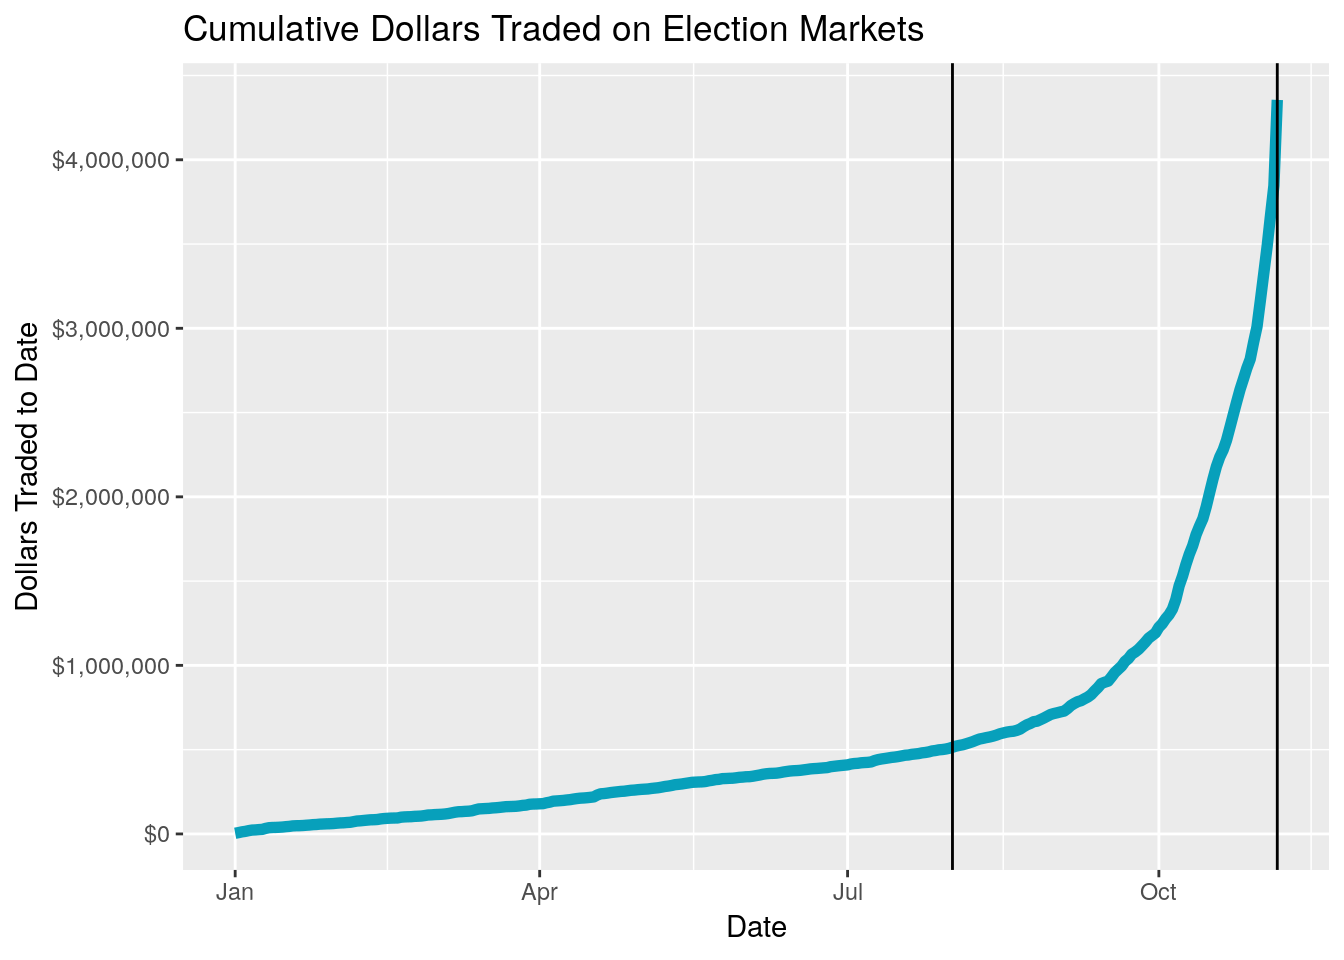
\includegraphics{code_files/figure-latex/unnamed-chunk-11-1.pdf}

\begin{Shaded}
\begin{Highlighting}[]
\CommentTok{# Number of polls conducted over time}
\NormalTok{polling }\OperatorTok
\StringTok{  }\KeywordTok{group_by}\NormalTok{(start_date) }\OperatorTok
\StringTok{  }\KeywordTok{summarise}\NormalTok{(}\DataTypeTok{n =} \KeywordTok{n}\NormalTok{()) }\OperatorTok
\StringTok{  }\KeywordTok{mutate}\NormalTok{(}\DataTypeTok{cumsum =} \KeywordTok{cumsum}\NormalTok{(n)) }\OperatorTok
\StringTok{  }\KeywordTok{filter}\NormalTok{(start_date }\OperatorTok{>=}\StringTok{ "2018-01-01"}\NormalTok{, start_date }\OperatorTok{<=}\StringTok{ "2018-11-05"}\NormalTok{) }\OperatorTok
\StringTok{  }\KeywordTok{ggplot}\NormalTok{(}\DataTypeTok{mapping =} \KeywordTok{aes}\NormalTok{(}\DataTypeTok{x =}\NormalTok{ start_date, }\DataTypeTok{y =}\NormalTok{ cumsum)) }\OperatorTok{+}
\StringTok{  }\KeywordTok{geom_line}\NormalTok{(}\DataTypeTok{color =}\NormalTok{ color_model, }\DataTypeTok{size =} \DecValTok{2}\NormalTok{) }\OperatorTok{+}
\StringTok{  }\KeywordTok{geom_vline}\NormalTok{(}\DataTypeTok{xintercept =} \KeywordTok{as.Date}\NormalTok{(}\StringTok{"2018-08-01"}\NormalTok{), }\DataTypeTok{size =} \FloatTok{0.5}\NormalTok{) }\OperatorTok{+}
\StringTok{  }\KeywordTok{geom_vline}\NormalTok{(}\DataTypeTok{xintercept =} \KeywordTok{as.Date}\NormalTok{(}\StringTok{"2018-11-04"}\NormalTok{), }\DataTypeTok{size =} \FloatTok{0.5}\NormalTok{) }\OperatorTok{+}
\StringTok{  }\KeywordTok{labs}\NormalTok{(}\DataTypeTok{title =} \StringTok{"Cumulative Number of Congressional Polls"}\NormalTok{,}
       \DataTypeTok{x =} \StringTok{"Date"}\NormalTok{,}
       \DataTypeTok{y =} \StringTok{"Polls to Date"}\NormalTok{)}
\end{Highlighting}
\end{Shaded}

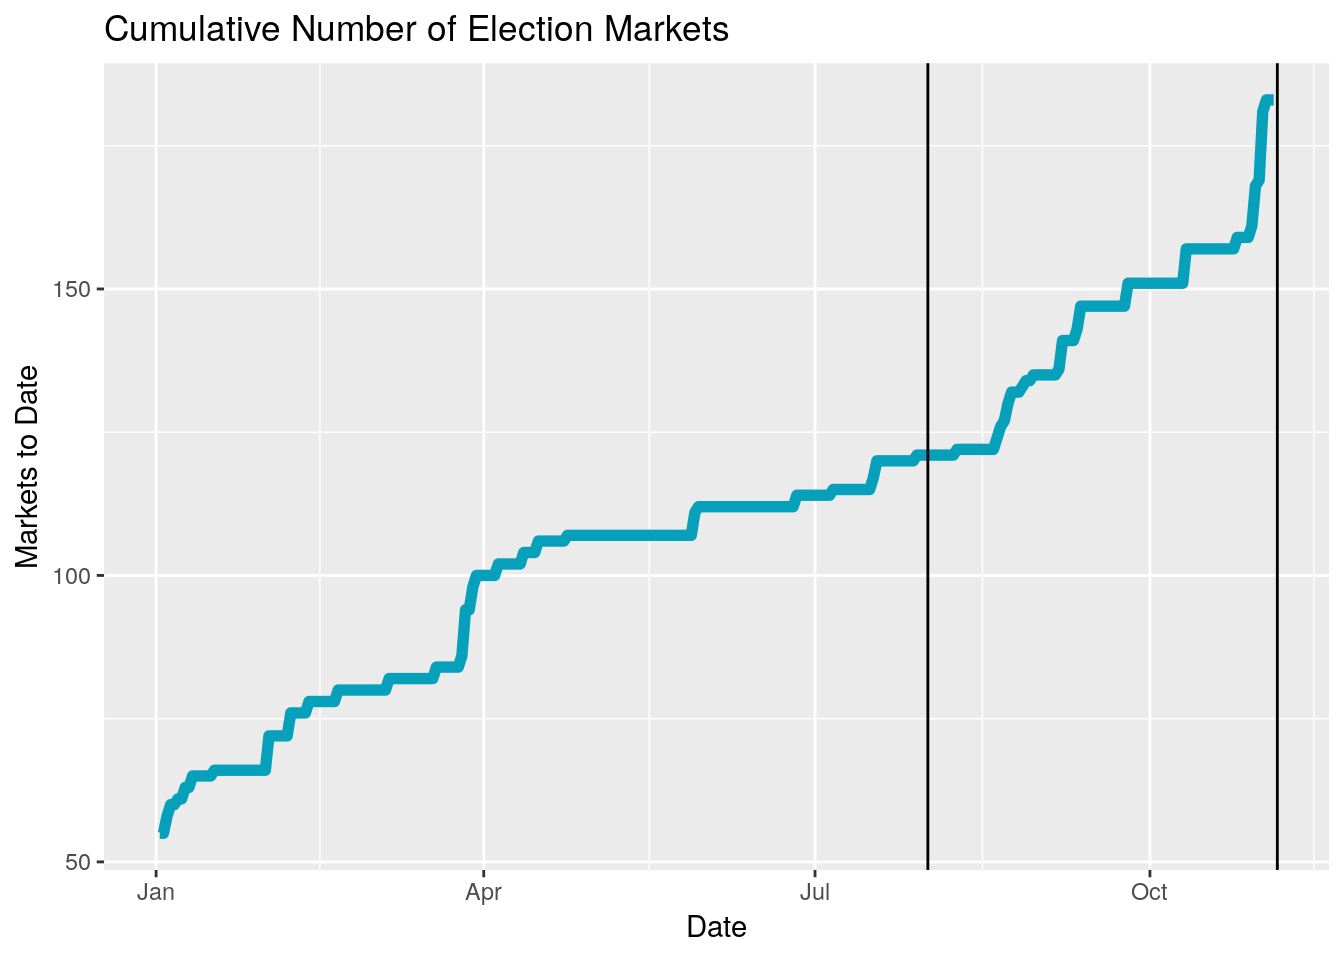
\includegraphics{code_files/figure-latex/unnamed-chunk-12-1.pdf}

\begin{Shaded}
\begin{Highlighting}[]
\CommentTok{# Number of dollars traded over time}
\NormalTok{markets }\OperatorTok
\StringTok{  }\KeywordTok{filter}\NormalTok{(date }\OperatorTok{>=}\StringTok{ "2018-01-01"}\NormalTok{, date }\OperatorTok{<=}\StringTok{ "2018-11-05"}\NormalTok{) }\OperatorTok
\StringTok{  }\KeywordTok{group_by}\NormalTok{(date) }\OperatorTok
\StringTok{  }\KeywordTok{mutate}\NormalTok{(}\DataTypeTok{traded =}\NormalTok{ close }\OperatorTok{*}\StringTok{ }\NormalTok{volume) }\OperatorTok
\StringTok{  }\KeywordTok{summarise}\NormalTok{(}\DataTypeTok{sum =} \KeywordTok{sum}\NormalTok{(traded, }\DataTypeTok{na.rm =} \OtherTok{TRUE}\NormalTok{)) }\OperatorTok
\StringTok{  }\KeywordTok{mutate}\NormalTok{(}\DataTypeTok{cumsum =} \KeywordTok{cumsum}\NormalTok{(sum)) }\OperatorTok
\StringTok{  }\KeywordTok{ggplot}\NormalTok{(}\DataTypeTok{mapping =} \KeywordTok{aes}\NormalTok{(}\DataTypeTok{x =}\NormalTok{ date, }\DataTypeTok{y =}\NormalTok{ cumsum)) }\OperatorTok{+}
\StringTok{  }\KeywordTok{geom_line}\NormalTok{(}\DataTypeTok{color =}\NormalTok{ color_market, }\DataTypeTok{size =} \DecValTok{2}\NormalTok{) }\OperatorTok{+}
\StringTok{  }\KeywordTok{geom_vline}\NormalTok{(}\DataTypeTok{xintercept =} \KeywordTok{as.Date}\NormalTok{(}\StringTok{"2018-08-01"}\NormalTok{), }\DataTypeTok{size =} \FloatTok{0.5}\NormalTok{) }\OperatorTok{+}
\StringTok{  }\KeywordTok{geom_vline}\NormalTok{(}\DataTypeTok{xintercept =} \KeywordTok{as.Date}\NormalTok{(}\StringTok{"2018-11-05"}\NormalTok{), }\DataTypeTok{size =} \FloatTok{0.5}\NormalTok{) }\OperatorTok{+}
\StringTok{  }\KeywordTok{scale_y_continuous}\NormalTok{(}\DataTypeTok{labels =}\NormalTok{ scales}\OperatorTok{::}\NormalTok{dollar) }\OperatorTok{+}
\StringTok{  }\KeywordTok{labs}\NormalTok{(}\DataTypeTok{title =} \StringTok{"Cumulative Dollars Traded on Election Markets"}\NormalTok{,}
       \DataTypeTok{x =} \StringTok{"Date"}\NormalTok{,}
       \DataTypeTok{y =} \StringTok{"Dollars Traded to Date"}\NormalTok{)}
\end{Highlighting}
\end{Shaded}

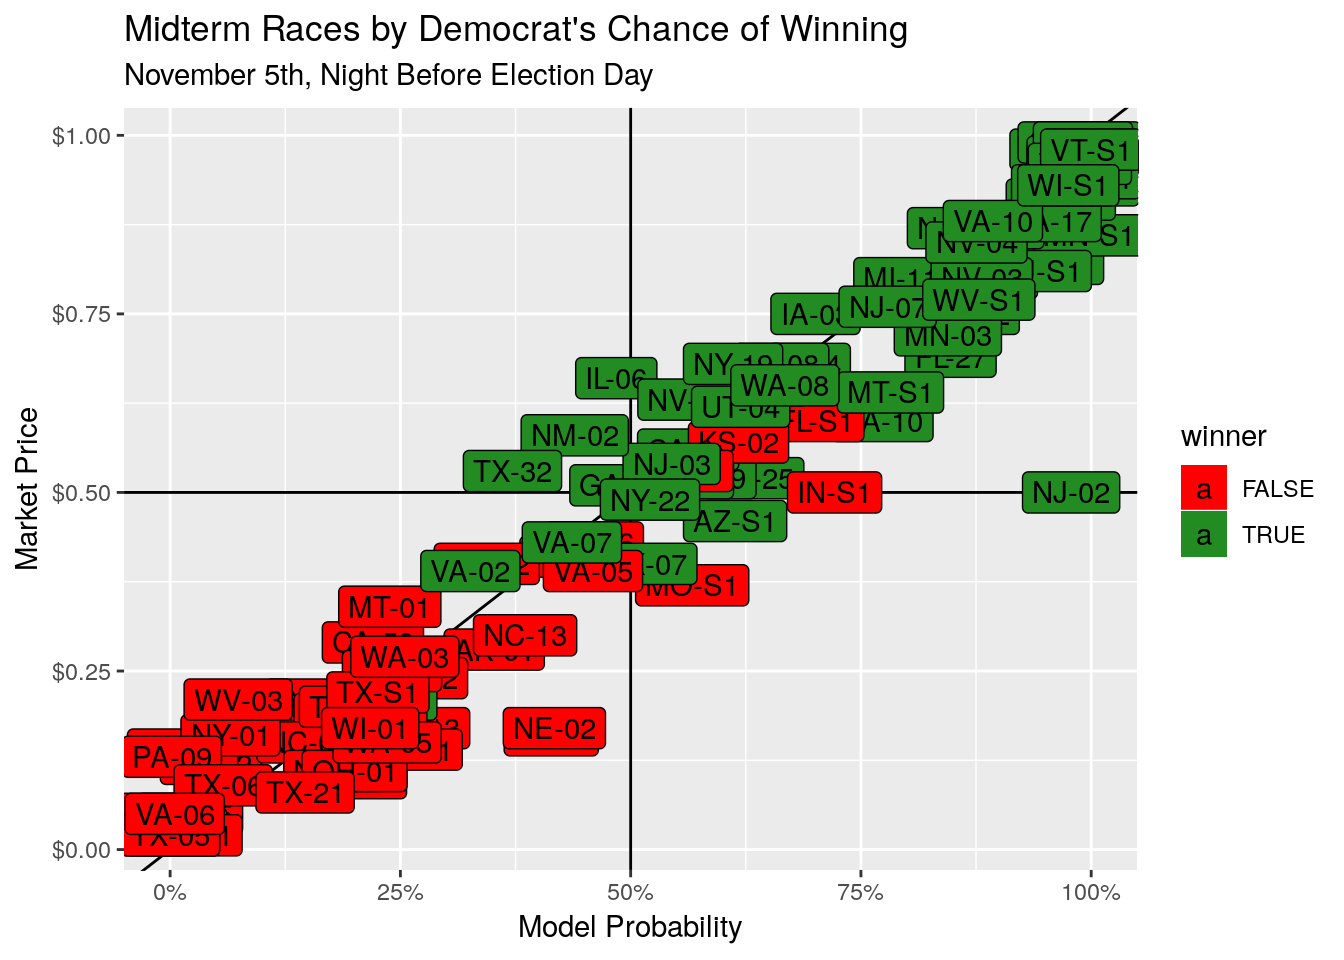
\includegraphics{code_files/figure-latex/unnamed-chunk-13-1.pdf}

\begin{Shaded}
\begin{Highlighting}[]
\CommentTok{# Number of markets opened over time}
\NormalTok{markets }\OperatorTok
\StringTok{  }\KeywordTok{filter}\NormalTok{(date }\OperatorTok{>}\StringTok{ "2018-01-01"}\NormalTok{, date }\OperatorTok{<}\StringTok{ "2018-11-05"}\NormalTok{) }\OperatorTok
\StringTok{  }\KeywordTok{group_by}\NormalTok{(date) }\OperatorTok
\StringTok{  }\KeywordTok{summarise}\NormalTok{(}\DataTypeTok{count =} \KeywordTok{n}\NormalTok{()) }\OperatorTok
\StringTok{  }\KeywordTok{ggplot}\NormalTok{(}\DataTypeTok{mapping =} \KeywordTok{aes}\NormalTok{(}\DataTypeTok{x =}\NormalTok{ date, }\DataTypeTok{y =}\NormalTok{ count)) }\OperatorTok{+}
\StringTok{  }\KeywordTok{geom_line}\NormalTok{(}\DataTypeTok{color =}\NormalTok{ color_market, }\DataTypeTok{size =} \DecValTok{2}\NormalTok{) }\OperatorTok{+}
\StringTok{  }\KeywordTok{geom_vline}\NormalTok{(}\DataTypeTok{xintercept =} \KeywordTok{as_date}\NormalTok{(}\StringTok{"2018-08-01"}\NormalTok{), }\DataTypeTok{size =} \FloatTok{0.5}\NormalTok{) }\OperatorTok{+}
\StringTok{  }\KeywordTok{geom_vline}\NormalTok{(}\DataTypeTok{xintercept =} \KeywordTok{as_date}\NormalTok{(}\StringTok{"2018-11-05"}\NormalTok{), }\DataTypeTok{size =} \FloatTok{0.5}\NormalTok{) }\OperatorTok{+}
\StringTok{  }\KeywordTok{labs}\NormalTok{(}\DataTypeTok{title =} \StringTok{"Cumulative Number of Election Markets"}\NormalTok{,}
       \DataTypeTok{x =} \StringTok{"Date"}\NormalTok{,}
       \DataTypeTok{y =} \StringTok{"Markets to Date"}\NormalTok{)}
\end{Highlighting}
\end{Shaded}

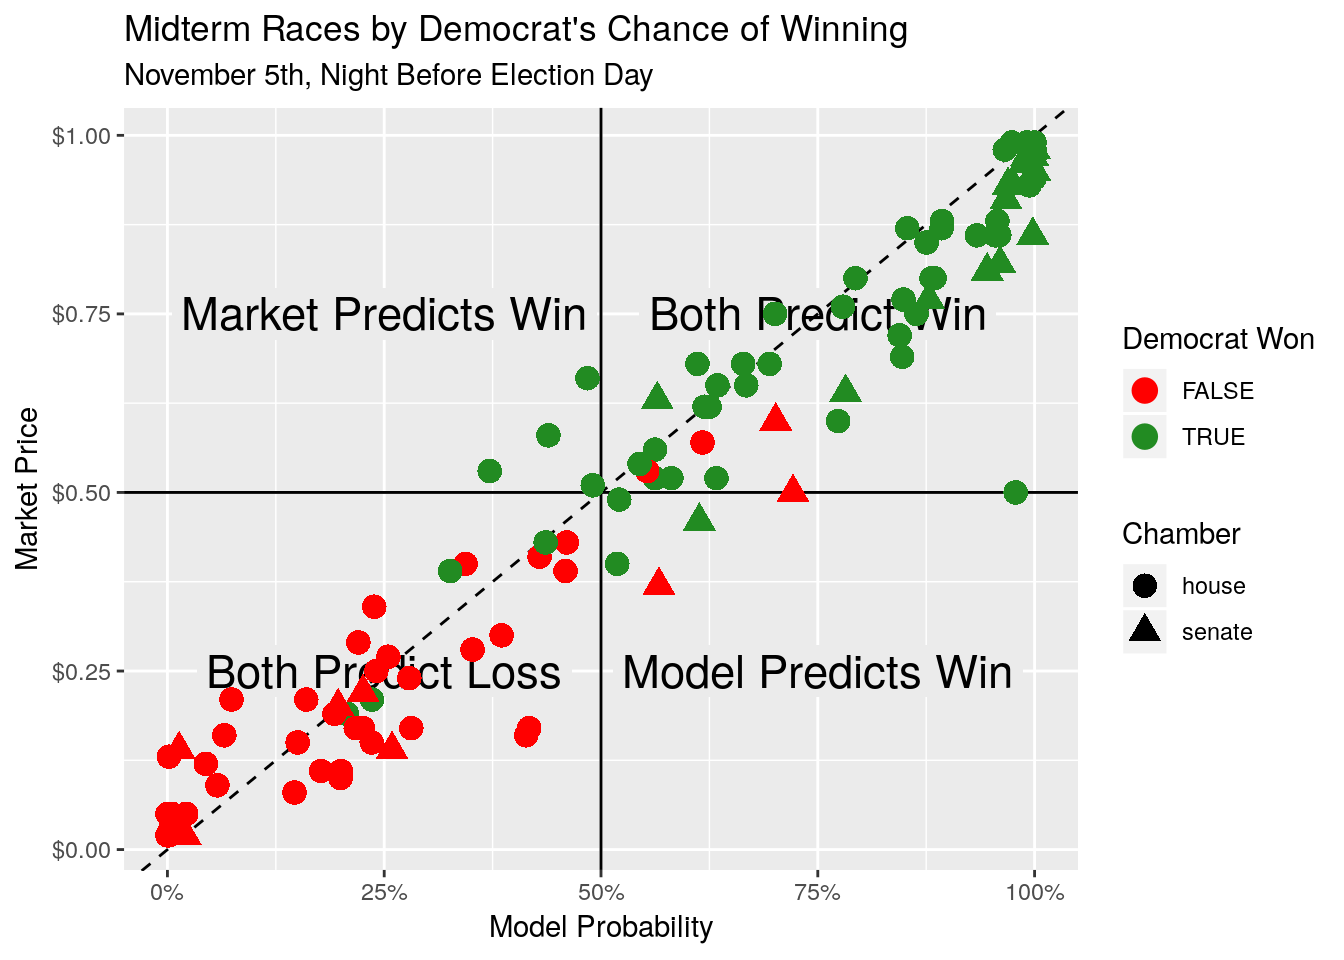
\includegraphics{code_files/figure-latex/unnamed-chunk-14-1.pdf}

\begin{Shaded}
\begin{Highlighting}[]
\CommentTok{# Races by Model on X and Market on Y}
\NormalTok{messy }\OperatorTok
\StringTok{  }\KeywordTok{mutate}\NormalTok{(}\DataTypeTok{party =} \StringTok{"D"}\NormalTok{) }\OperatorTok
\StringTok{  }\KeywordTok{filter}\NormalTok{(date }\OperatorTok{==}\StringTok{ "2018-11-05"}\NormalTok{) }\OperatorTok
\StringTok{  }\KeywordTok{left_join}\NormalTok{(model, }\DataTypeTok{by =} \KeywordTok{c}\NormalTok{(}\StringTok{"date"}\NormalTok{, }\StringTok{"race"}\NormalTok{, }\StringTok{"party"}\NormalTok{)) }\OperatorTok
\StringTok{  }\KeywordTok{inner_join}\NormalTok{(results, }\DataTypeTok{by =} \StringTok{"race"}\NormalTok{) }\OperatorTok
\StringTok{  }\KeywordTok{ggplot}\NormalTok{(}\KeywordTok{aes}\NormalTok{(}\DataTypeTok{x  =}\NormalTok{ model, }\DataTypeTok{y  =}\NormalTok{ market)) }\OperatorTok{+}
\StringTok{  }\KeywordTok{geom_hline}\NormalTok{(}\DataTypeTok{yintercept =} \FloatTok{0.5}\NormalTok{) }\OperatorTok{+}
\StringTok{  }\KeywordTok{geom_vline}\NormalTok{(}\DataTypeTok{xintercept =} \FloatTok{0.5}\NormalTok{) }\OperatorTok{+}
\StringTok{  }\KeywordTok{geom_abline}\NormalTok{(}\DataTypeTok{slope =} \DecValTok{1}\NormalTok{, }\DataTypeTok{intercept =} \DecValTok{0}\NormalTok{) }\OperatorTok{+}
\StringTok{  }\KeywordTok{geom_label}\NormalTok{(}\KeywordTok{aes}\NormalTok{(}\DataTypeTok{fill =}\NormalTok{ winner, }\DataTypeTok{label =}\NormalTok{ race)) }\OperatorTok{+}
\StringTok{  }\KeywordTok{scale_y_continuous}\NormalTok{(}\DataTypeTok{labels =}\NormalTok{ scales}\OperatorTok{::}\NormalTok{dollar) }\OperatorTok{+}
\StringTok{  }\KeywordTok{scale_x_continuous}\NormalTok{(}\DataTypeTok{labels =}\NormalTok{ scales}\OperatorTok{::}\NormalTok{percent) }\OperatorTok{+}
\StringTok{  }\KeywordTok{scale_fill_manual}\NormalTok{(}\DataTypeTok{values =} \KeywordTok{c}\NormalTok{(}\StringTok{"red"}\NormalTok{, }\StringTok{"forestgreen"}\NormalTok{)) }\OperatorTok{+}
\StringTok{  }\KeywordTok{labs}\NormalTok{(}\DataTypeTok{title =} \StringTok{"Midterm Races by Democrat's Chance of Winning"}\NormalTok{,}
       \DataTypeTok{subtitle =} \StringTok{"November 5th, Night Before Election Day"}\NormalTok{,}
       \DataTypeTok{x =} \StringTok{"Model Probability"}\NormalTok{,}
       \DataTypeTok{y =} \StringTok{"Market Price"}\NormalTok{,}
       \DataTypeTok{shape =} \StringTok{"Chamber"}\NormalTok{,}
       \DataTypeTok{color =} \StringTok{"Incumbency"}\NormalTok{)}
\end{Highlighting}
\end{Shaded}

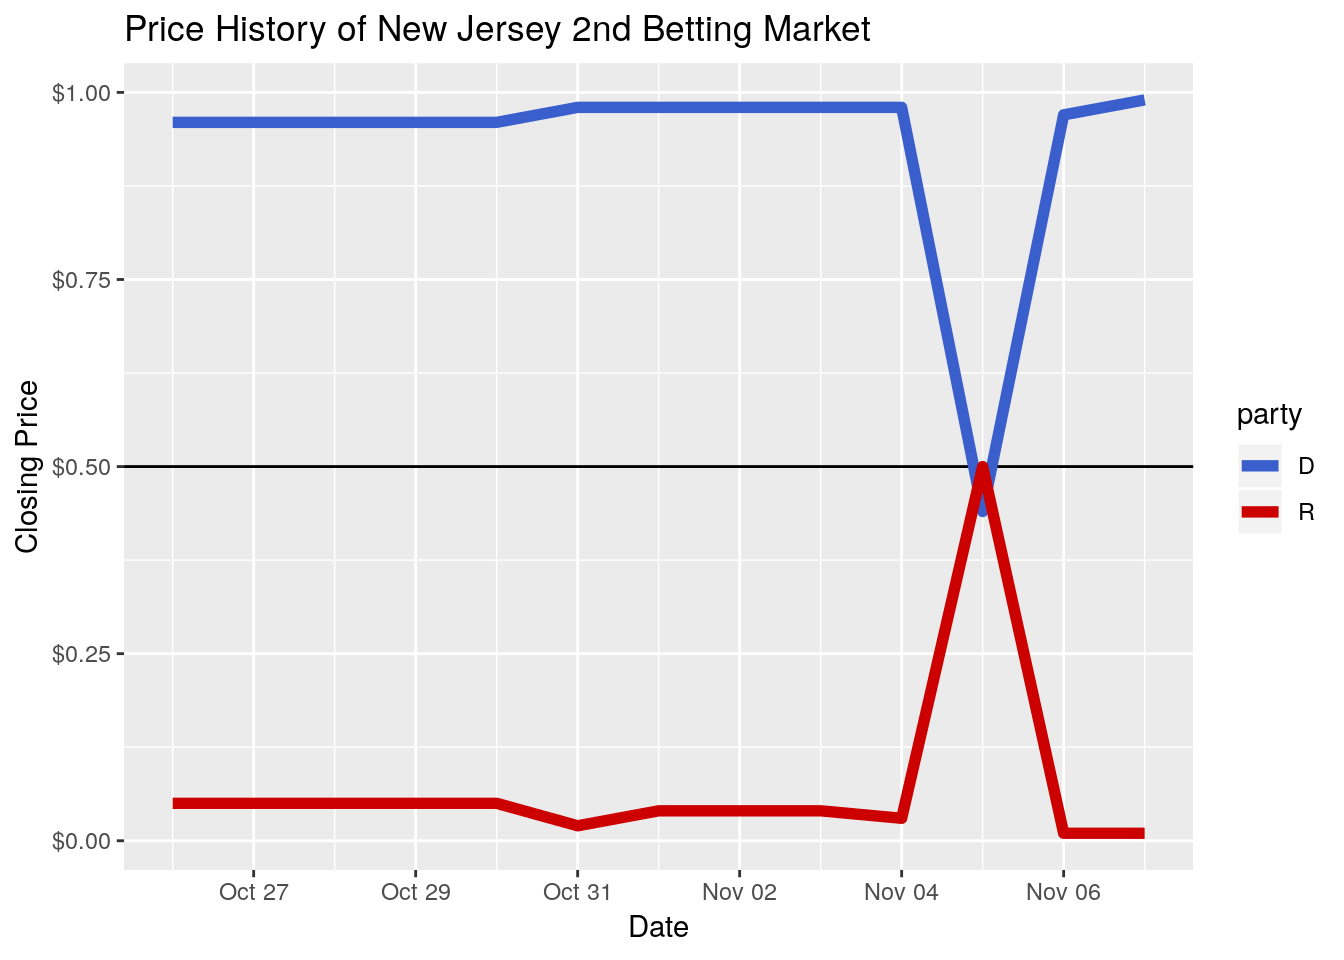
\includegraphics{code_files/figure-latex/unnamed-chunk-15-1.pdf}

\begin{Shaded}
\begin{Highlighting}[]
\NormalTok{messy }\OperatorTok
\StringTok{  }\KeywordTok{mutate}\NormalTok{(}\DataTypeTok{party =} \StringTok{"D"}\NormalTok{) }\OperatorTok
\StringTok{  }\KeywordTok{filter}\NormalTok{(date }\OperatorTok{==}\StringTok{ "2018-11-05"}\NormalTok{) }\OperatorTok
\StringTok{  }\KeywordTok{left_join}\NormalTok{(model, }\DataTypeTok{by =} \KeywordTok{c}\NormalTok{(}\StringTok{"date"}\NormalTok{, }\StringTok{"race"}\NormalTok{, }\StringTok{"party"}\NormalTok{)) }\OperatorTok
\StringTok{  }\KeywordTok{inner_join}\NormalTok{(results, }\DataTypeTok{by =} \StringTok{"race"}\NormalTok{) }\OperatorTok
\StringTok{  }\KeywordTok{ggplot}\NormalTok{(}\KeywordTok{aes}\NormalTok{(}\DataTypeTok{x  =}\NormalTok{ model, }\DataTypeTok{y  =}\NormalTok{ market)) }\OperatorTok{+}
\StringTok{  }\KeywordTok{geom_hline}\NormalTok{(}\DataTypeTok{yintercept =} \FloatTok{0.5}\NormalTok{) }\OperatorTok{+}
\StringTok{  }\KeywordTok{geom_vline}\NormalTok{(}\DataTypeTok{xintercept =} \FloatTok{0.5}\NormalTok{) }\OperatorTok{+}
\StringTok{  }\KeywordTok{geom_label}\NormalTok{(}\DataTypeTok{mapping =} \KeywordTok{aes}\NormalTok{(}\DataTypeTok{x =} \FloatTok{0.25}\NormalTok{, }\DataTypeTok{y =} \FloatTok{0.75}\NormalTok{, }\DataTypeTok{label =} \StringTok{"Market Predicts Win"}\NormalTok{),}
             \DataTypeTok{label.size =} \DecValTok{0}\NormalTok{,}
             \DataTypeTok{fill =} \StringTok{"#ebebeb"}\NormalTok{,}
             \DataTypeTok{size =} \DecValTok{6}\NormalTok{) }\OperatorTok{+}
\StringTok{  }\KeywordTok{geom_label}\NormalTok{(}\DataTypeTok{mapping =} \KeywordTok{aes}\NormalTok{(}\DataTypeTok{x =} \FloatTok{0.75}\NormalTok{, }\DataTypeTok{y =} \FloatTok{0.25}\NormalTok{, }\DataTypeTok{label =} \StringTok{"Model Predicts Win"}\NormalTok{),}
             \DataTypeTok{label.size =} \DecValTok{0}\NormalTok{,}
             \DataTypeTok{fill =} \StringTok{"#ebebeb"}\NormalTok{,}
             \DataTypeTok{size =} \DecValTok{6}\NormalTok{) }\OperatorTok{+}
\StringTok{  }\KeywordTok{geom_label}\NormalTok{(}\DataTypeTok{mapping =} \KeywordTok{aes}\NormalTok{(}\DataTypeTok{x =} \FloatTok{0.25}\NormalTok{, }\DataTypeTok{y =} \FloatTok{0.25}\NormalTok{, }\DataTypeTok{label =} \StringTok{"Both Predict Loss"}\NormalTok{),}
             \DataTypeTok{label.size =} \DecValTok{0}\NormalTok{,}
             \DataTypeTok{fill =} \StringTok{"#ebebeb"}\NormalTok{,}
             \DataTypeTok{size =} \DecValTok{6}\NormalTok{) }\OperatorTok{+}
\StringTok{  }\KeywordTok{geom_label}\NormalTok{(}\DataTypeTok{mapping =} \KeywordTok{aes}\NormalTok{(}\DataTypeTok{x =} \FloatTok{0.75}\NormalTok{, }\DataTypeTok{y =} \FloatTok{0.75}\NormalTok{, }\DataTypeTok{label =} \StringTok{"Both Predict Win"}\NormalTok{),}
             \DataTypeTok{label.size =} \DecValTok{0}\NormalTok{,}
             \DataTypeTok{fill =} \StringTok{"#ebebeb"}\NormalTok{,}
             \DataTypeTok{size =} \DecValTok{6}\NormalTok{) }\OperatorTok{+}
\StringTok{  }\KeywordTok{geom_abline}\NormalTok{(}\DataTypeTok{slope =} \DecValTok{1}\NormalTok{, }\DataTypeTok{intercept =} \DecValTok{0}\NormalTok{, }\DataTypeTok{lty =} \DecValTok{2}\NormalTok{) }\OperatorTok{+}
\StringTok{  }\KeywordTok{geom_point}\NormalTok{(}\KeywordTok{aes}\NormalTok{(}\DataTypeTok{color =}\NormalTok{ winner, }\DataTypeTok{shape =}\NormalTok{ chamber), }\DataTypeTok{size =} \DecValTok{4}\NormalTok{) }\OperatorTok{+}
\StringTok{  }\KeywordTok{scale_y_continuous}\NormalTok{(}\DataTypeTok{labels =}\NormalTok{ scales}\OperatorTok{::}\NormalTok{dollar) }\OperatorTok{+}
\StringTok{  }\KeywordTok{scale_x_continuous}\NormalTok{(}\DataTypeTok{labels =}\NormalTok{ scales}\OperatorTok{::}\NormalTok{percent) }\OperatorTok{+}
\StringTok{  }\KeywordTok{scale_color_manual}\NormalTok{(}\DataTypeTok{values =} \KeywordTok{c}\NormalTok{(}\StringTok{"red"}\NormalTok{, }\StringTok{"forestgreen"}\NormalTok{)) }\OperatorTok{+}
\StringTok{  }\KeywordTok{labs}\NormalTok{(}\DataTypeTok{title =} \StringTok{"Midterm Races by Democrat's Chance of Winning"}\NormalTok{,}
       \DataTypeTok{subtitle =} \StringTok{"November 5th, Night Before Election Day"}\NormalTok{,}
       \DataTypeTok{x =} \StringTok{"Model Probability"}\NormalTok{,}
       \DataTypeTok{y =} \StringTok{"Market Price"}\NormalTok{,}
       \DataTypeTok{shape =} \StringTok{"Chamber"}\NormalTok{,}
       \DataTypeTok{color =} \StringTok{"Democrat Won"}\NormalTok{)}
\end{Highlighting}
\end{Shaded}

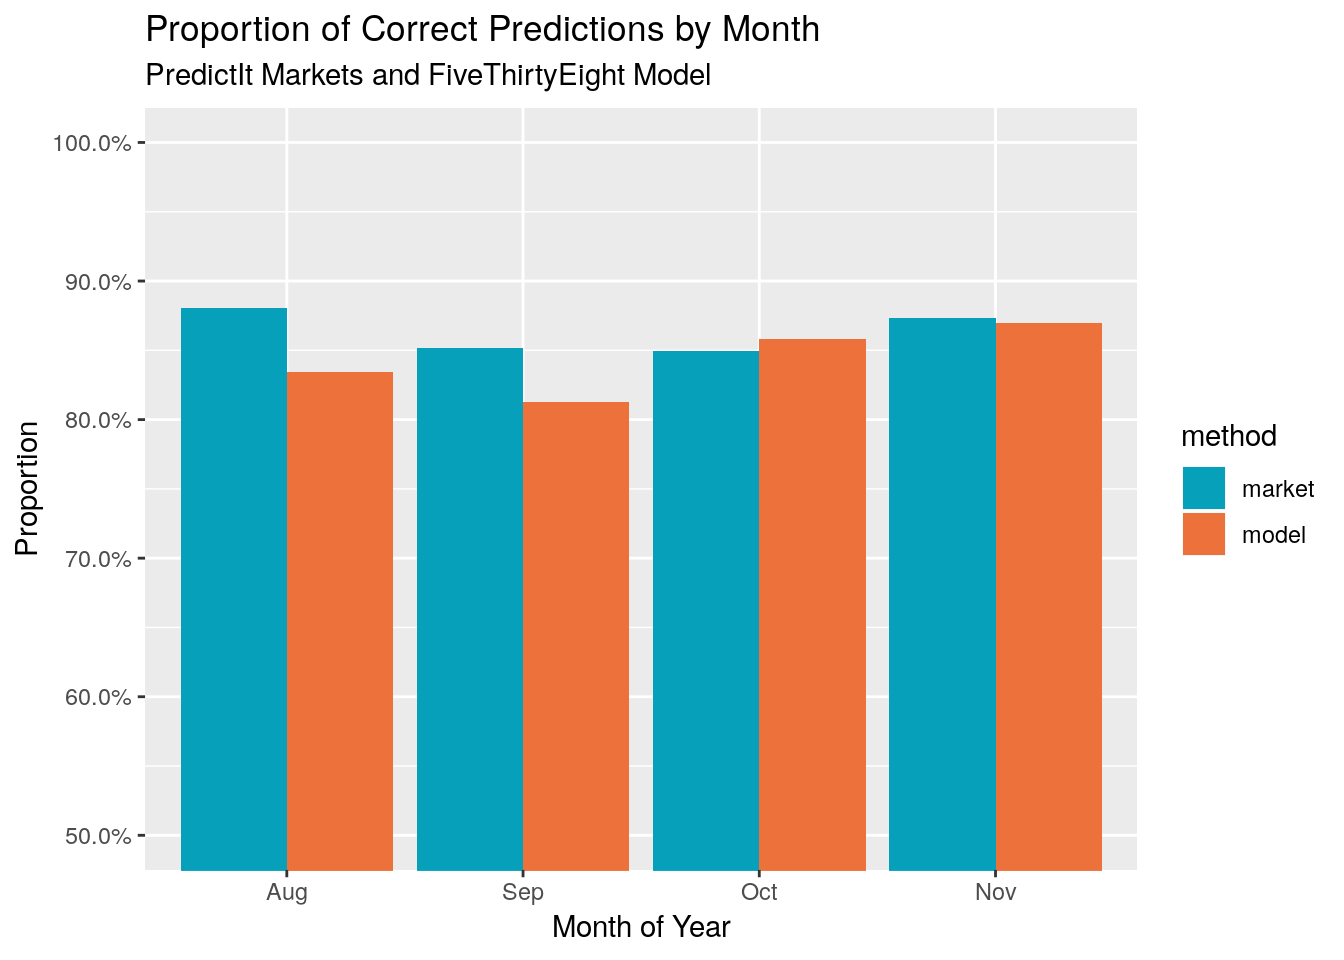
\includegraphics{code_files/figure-latex/unnamed-chunk-16-1.pdf}

\begin{Shaded}
\begin{Highlighting}[]
\CommentTok{# Weird NJ-02 Market Error}
\NormalTok{markets }\OperatorTok
\StringTok{  }\KeywordTok{filter}\NormalTok{(race }\OperatorTok{==}\StringTok{ "NJ-02"}\NormalTok{, date }\OperatorTok{>}\StringTok{ "2018-10-25"}\NormalTok{) }\OperatorTok
\StringTok{  }\KeywordTok{ggplot}\NormalTok{(}\KeywordTok{aes}\NormalTok{(}\DataTypeTok{x =}\NormalTok{ date, }\DataTypeTok{y =}\NormalTok{ close)) }\OperatorTok{+}
\StringTok{  }\KeywordTok{geom_hline}\NormalTok{(}\DataTypeTok{yintercept =} \FloatTok{0.5}\NormalTok{) }\OperatorTok{+}
\StringTok{  }\KeywordTok{geom_line}\NormalTok{(}\KeywordTok{aes}\NormalTok{(}\DataTypeTok{color =}\NormalTok{ party), }\DataTypeTok{size =} \DecValTok{2}\NormalTok{) }\OperatorTok{+}
\StringTok{  }\KeywordTok{scale_color_manual}\NormalTok{(}\DataTypeTok{values =} \KeywordTok{c}\NormalTok{(color_blue, color_red)) }\OperatorTok{+}
\StringTok{  }\KeywordTok{scale_y_continuous}\NormalTok{(}\DataTypeTok{labels =}\NormalTok{ scales}\OperatorTok{::}\NormalTok{dollar) }\OperatorTok{+}
\StringTok{  }\KeywordTok{scale_x_date}\NormalTok{() }\OperatorTok{+}
\StringTok{  }\KeywordTok{labs}\NormalTok{(}\DataTypeTok{title =} \StringTok{"Price History of New Jersey 2nd Betting Market"}\NormalTok{,}
       \DataTypeTok{x =} \StringTok{"Date"}\NormalTok{,}
       \DataTypeTok{y =} \StringTok{"Closing Price"}\NormalTok{)}
\end{Highlighting}
\end{Shaded}

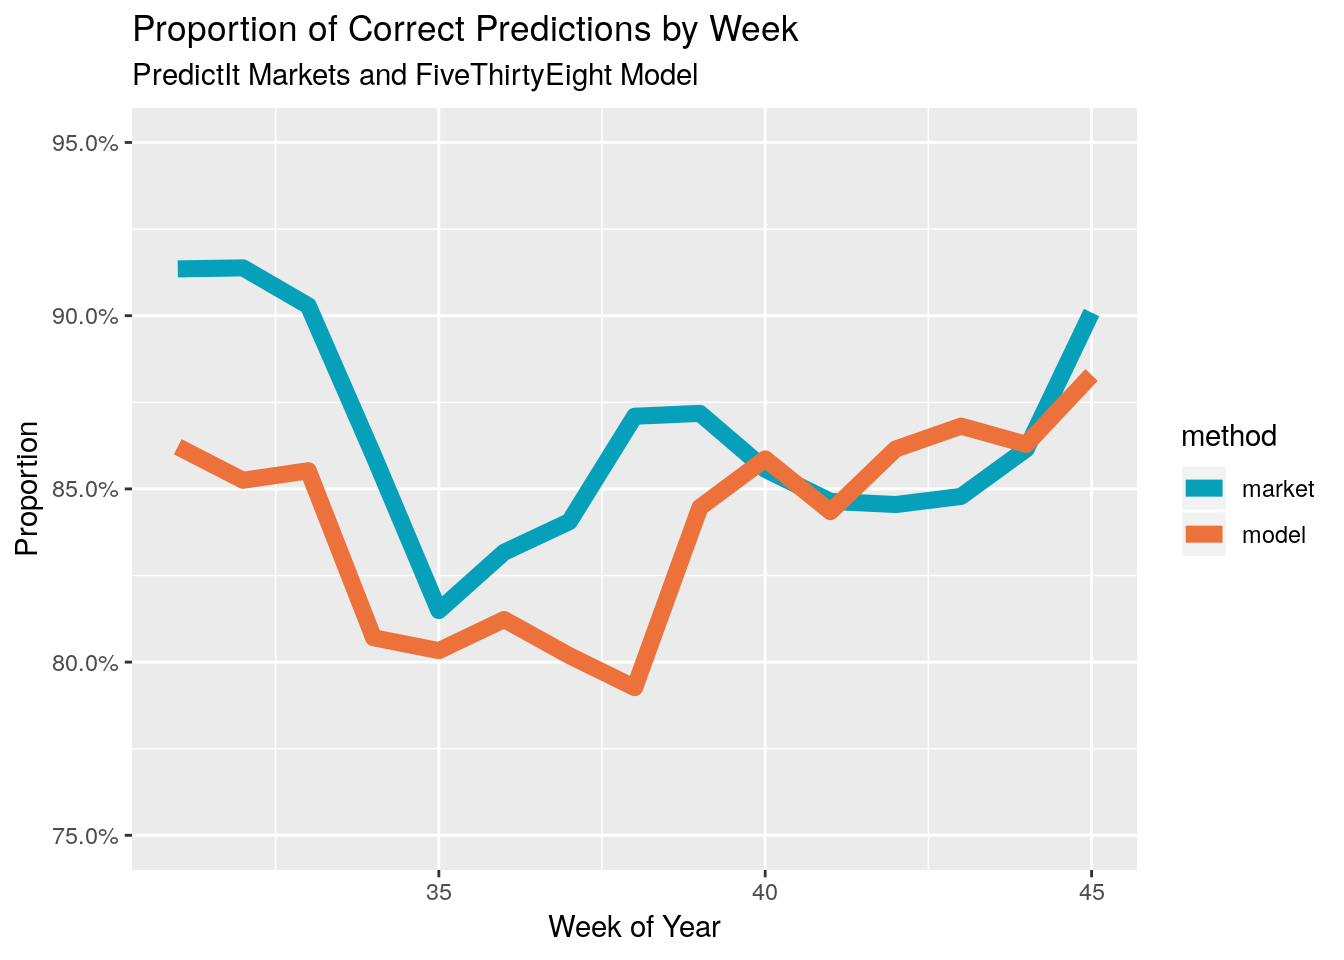
\includegraphics{code_files/figure-latex/unnamed-chunk-17-1.pdf}

\begin{Shaded}
\begin{Highlighting}[]
\NormalTok{hits }\OperatorTok
\StringTok{  }\KeywordTok{mutate}\NormalTok{(}\DataTypeTok{month =} \KeywordTok{month}\NormalTok{(date, }\DataTypeTok{label =} \OtherTok{TRUE}\NormalTok{)) }\OperatorTok
\StringTok{  }\KeywordTok{group_by}\NormalTok{(month, method) }\OperatorTok
\StringTok{  }\KeywordTok{summarise}\NormalTok{(}\DataTypeTok{prop =} \KeywordTok{mean}\NormalTok{(hit, }\DataTypeTok{na.rm =} \OtherTok{TRUE}\NormalTok{)) }\OperatorTok
\StringTok{  }\KeywordTok{ggplot}\NormalTok{(}\KeywordTok{aes}\NormalTok{(}\DataTypeTok{x =}\NormalTok{ month, }\DataTypeTok{y =}\NormalTok{ prop, }\DataTypeTok{fill =}\NormalTok{ method)) }\OperatorTok{+}
\StringTok{  }\KeywordTok{geom_col}\NormalTok{(}\DataTypeTok{position =} \StringTok{"dodge"}\NormalTok{) }\OperatorTok{+}
\StringTok{  }\KeywordTok{scale_fill_manual}\NormalTok{(}\DataTypeTok{values =} \KeywordTok{c}\NormalTok{(color_market, color_model)) }\OperatorTok{+}
\StringTok{  }\KeywordTok{coord_cartesian}\NormalTok{(}\DataTypeTok{ylim =} \KeywordTok{c}\NormalTok{(}\FloatTok{0.50}\NormalTok{, }\FloatTok{1.0}\NormalTok{)) }\OperatorTok{+}
\StringTok{  }\KeywordTok{scale_y_continuous}\NormalTok{(}\DataTypeTok{labels =}\NormalTok{ scales}\OperatorTok{::}\NormalTok{percent) }\OperatorTok{+}
\StringTok{  }\KeywordTok{labs}\NormalTok{(}\DataTypeTok{title =} \StringTok{"Proportion of Correct Predictions by Month"}\NormalTok{,}
       \DataTypeTok{subtitle =} \StringTok{"PredictIt Markets and FiveThirtyEight Model"}\NormalTok{,}
       \DataTypeTok{y =} \StringTok{"Proportion"}\NormalTok{,}
       \DataTypeTok{x =} \StringTok{"Month of Year"}\NormalTok{)}
\end{Highlighting}
\end{Shaded}

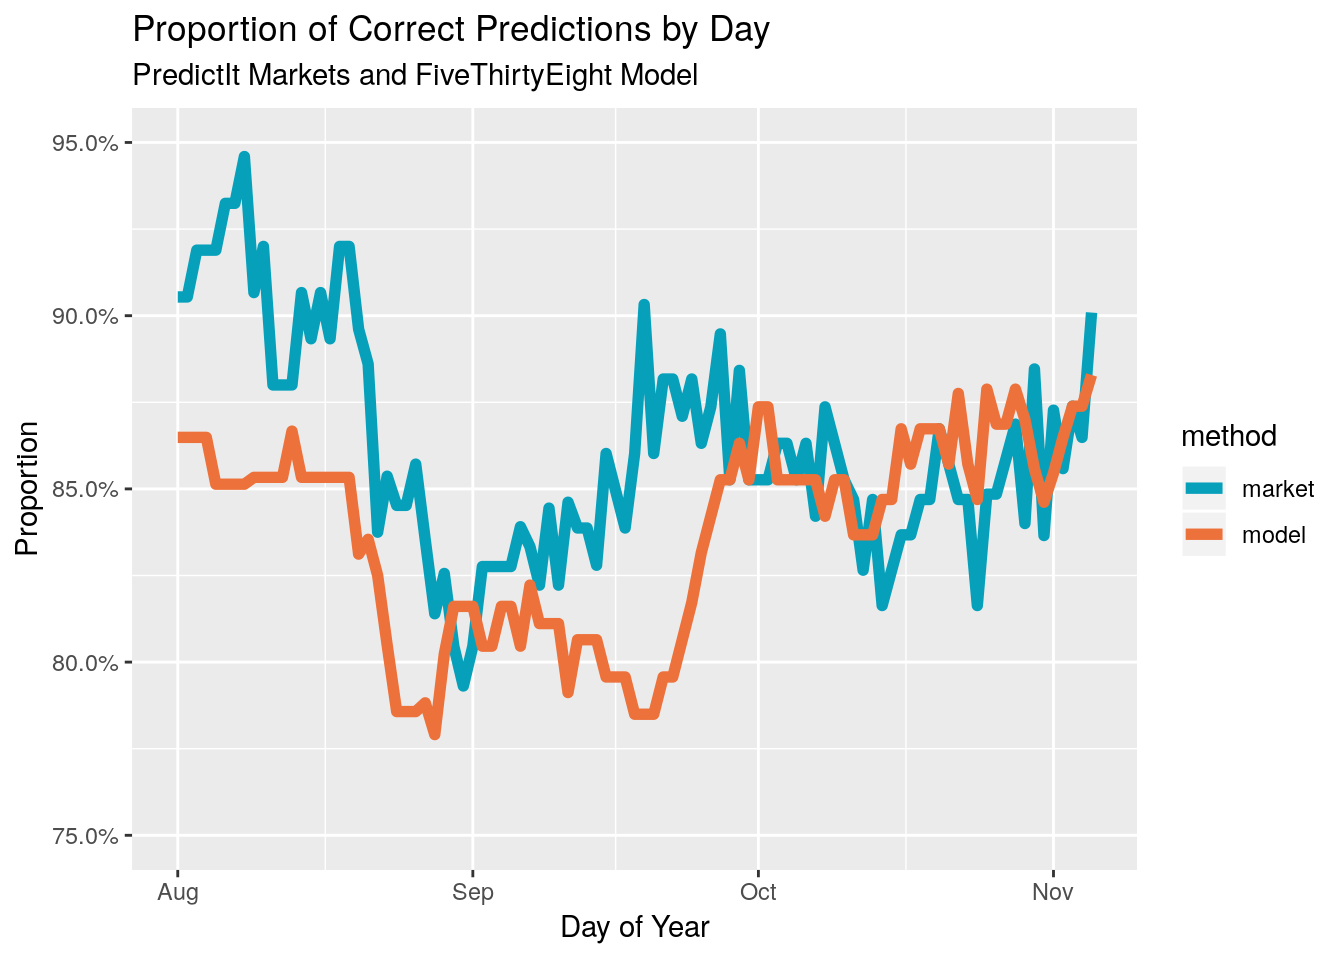
\includegraphics{code_files/figure-latex/unnamed-chunk-18-1.pdf}

\begin{Shaded}
\begin{Highlighting}[]
\NormalTok{hits }\OperatorTok
\StringTok{  }\KeywordTok{mutate}\NormalTok{(}\DataTypeTok{week =} \KeywordTok{week}\NormalTok{(date)) }\OperatorTok
\StringTok{  }\KeywordTok{group_by}\NormalTok{(week, method) }\OperatorTok
\StringTok{  }\KeywordTok{summarise}\NormalTok{(}\DataTypeTok{prop =} \KeywordTok{mean}\NormalTok{(hit, }\DataTypeTok{na.rm =} \OtherTok{TRUE}\NormalTok{)) }\OperatorTok
\StringTok{  }\KeywordTok{ggplot}\NormalTok{(}\KeywordTok{aes}\NormalTok{(}\DataTypeTok{x =}\NormalTok{ week, }\DataTypeTok{y =}\NormalTok{ prop, }\DataTypeTok{color =}\NormalTok{ method)) }\OperatorTok{+}
\StringTok{  }\KeywordTok{geom_line}\NormalTok{(}\DataTypeTok{size =} \DecValTok{3}\NormalTok{) }\OperatorTok{+}
\StringTok{  }\KeywordTok{coord_cartesian}\NormalTok{(}\DataTypeTok{ylim =} \KeywordTok{c}\NormalTok{(}\FloatTok{0.75}\NormalTok{, }\FloatTok{0.95}\NormalTok{)) }\OperatorTok{+}
\StringTok{  }\KeywordTok{scale_y_continuous}\NormalTok{(}\DataTypeTok{labels =}\NormalTok{ scales}\OperatorTok{::}\NormalTok{percent) }\OperatorTok{+}
\StringTok{  }\KeywordTok{scale_color_manual}\NormalTok{(}\DataTypeTok{values =} \KeywordTok{c}\NormalTok{(color_market, color_model)) }\OperatorTok{+}
\StringTok{  }\KeywordTok{labs}\NormalTok{(}\DataTypeTok{title =} \StringTok{"Proportion of Correct Predictions by Week"}\NormalTok{,}
       \DataTypeTok{subtitle =} \StringTok{"PredictIt Markets and FiveThirtyEight Model"}\NormalTok{,}
       \DataTypeTok{y =} \StringTok{"Proportion"}\NormalTok{,}
       \DataTypeTok{x =} \StringTok{"Week of Year"}\NormalTok{)}
\end{Highlighting}
\end{Shaded}

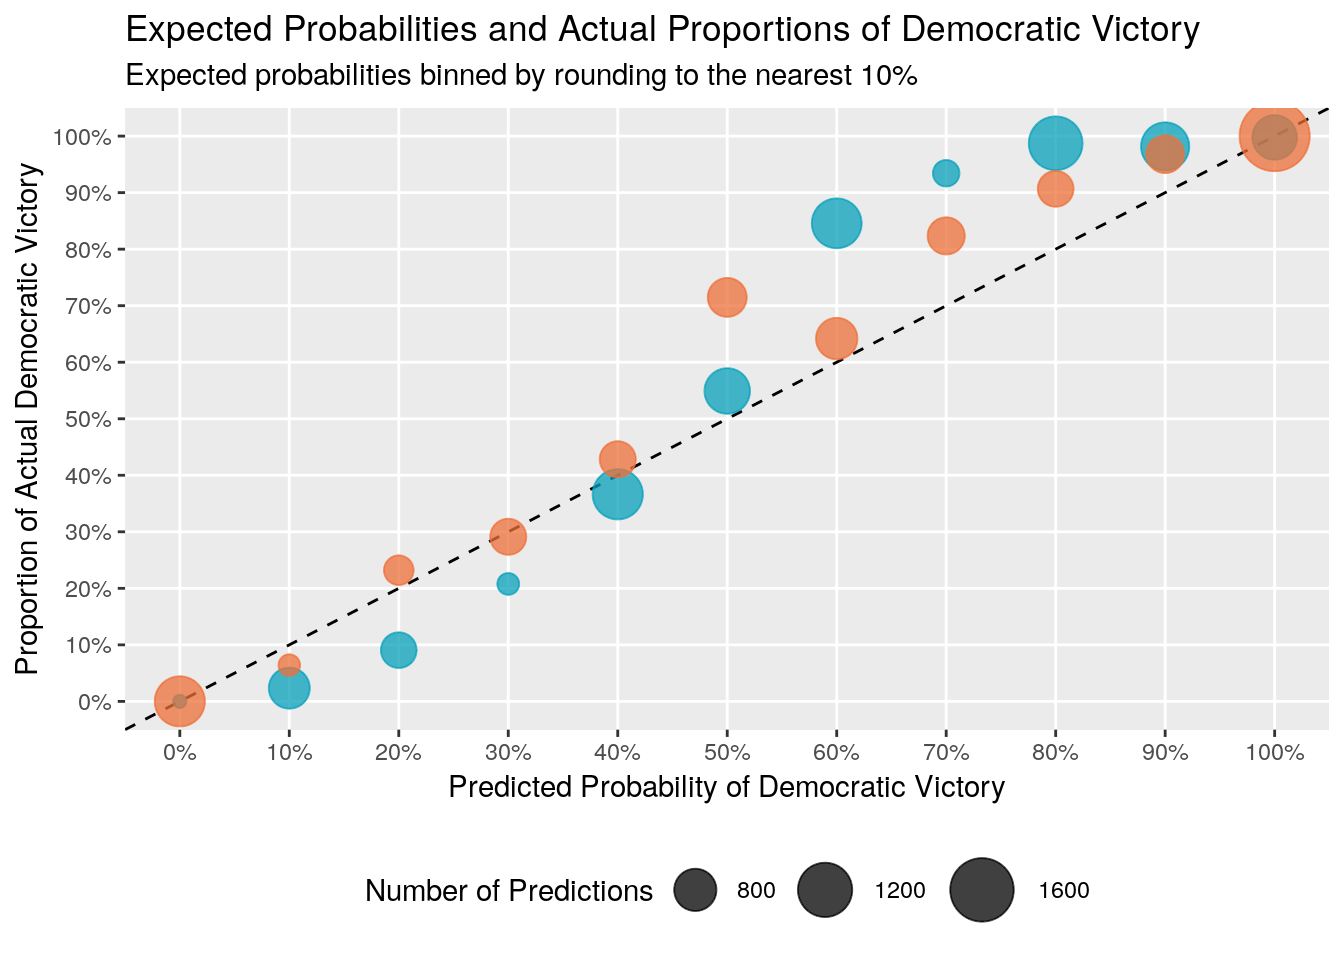
\includegraphics{code_files/figure-latex/unnamed-chunk-19-1.pdf}

\begin{Shaded}
\begin{Highlighting}[]
\NormalTok{hits }\OperatorTok
\StringTok{  }\KeywordTok{group_by}\NormalTok{(date, method) }\OperatorTok
\StringTok{  }\KeywordTok{summarise}\NormalTok{(}\DataTypeTok{prop =} \KeywordTok{mean}\NormalTok{(hit, }\DataTypeTok{na.rm =} \OtherTok{TRUE}\NormalTok{)) }\OperatorTok
\StringTok{  }\KeywordTok{ggplot}\NormalTok{(}\KeywordTok{aes}\NormalTok{(}\DataTypeTok{x =}\NormalTok{ date, }\DataTypeTok{y =}\NormalTok{ prop, }\DataTypeTok{color =}\NormalTok{ method)) }\OperatorTok{+}
\StringTok{  }\KeywordTok{geom_line}\NormalTok{(}\DataTypeTok{size =} \DecValTok{2}\NormalTok{) }\OperatorTok{+}
\StringTok{  }\KeywordTok{coord_cartesian}\NormalTok{(}\DataTypeTok{ylim =} \KeywordTok{c}\NormalTok{(}\FloatTok{0.75}\NormalTok{, }\FloatTok{0.95}\NormalTok{)) }\OperatorTok{+}
\StringTok{  }\KeywordTok{scale_y_continuous}\NormalTok{(}\DataTypeTok{labels =}\NormalTok{ scales}\OperatorTok{::}\NormalTok{percent) }\OperatorTok{+}
\StringTok{  }\KeywordTok{scale_color_manual}\NormalTok{(}\DataTypeTok{values =} \KeywordTok{c}\NormalTok{(color_market, color_model)) }\OperatorTok{+}
\StringTok{  }\KeywordTok{labs}\NormalTok{(}\DataTypeTok{title =} \StringTok{"Proportion of Correct Predictions by Day"}\NormalTok{,}
       \DataTypeTok{subtitle =} \StringTok{"PredictIt Markets and FiveThirtyEight Model"}\NormalTok{,}
       \DataTypeTok{y =} \StringTok{"Proportion"}\NormalTok{,}
       \DataTypeTok{x =} \StringTok{"Day of Year"}\NormalTok{)}
\end{Highlighting}
\end{Shaded}

\includegraphics{code_files/figure-latex/unnamed-chunk-20-1.pdf}

\begin{Shaded}
\begin{Highlighting}[]
\NormalTok{hits }\OperatorTok
\StringTok{  }\KeywordTok{mutate}\NormalTok{(}\DataTypeTok{bin =}\NormalTok{ prob }\OperatorTok\StringTok{ }\KeywordTok{round}\NormalTok{(}\DataTypeTok{digits =} \DecValTok{1}\NormalTok{)) }\OperatorTok
\StringTok{  }\KeywordTok{group_by}\NormalTok{(method, bin) }\OperatorTok
\StringTok{  }\KeywordTok{summarise}\NormalTok{(}\DataTypeTok{prop =} \KeywordTok{mean}\NormalTok{(winner), }\DataTypeTok{n =} \KeywordTok{n}\NormalTok{()) }\OperatorTok
\StringTok{  }\KeywordTok{ggplot}\NormalTok{(}\DataTypeTok{mapping =} \KeywordTok{aes}\NormalTok{(bin, prop)) }\OperatorTok{+}
\StringTok{  }\KeywordTok{geom_abline}\NormalTok{(}\DataTypeTok{intercept =} \DecValTok{0}\NormalTok{, }\DataTypeTok{slope =} \DecValTok{1}\NormalTok{, }\DataTypeTok{lty =} \DecValTok{2}\NormalTok{)  }\OperatorTok{+}
\StringTok{  }\KeywordTok{geom_point}\NormalTok{(}\DataTypeTok{mapping =} \KeywordTok{aes}\NormalTok{(}\DataTypeTok{color =}\NormalTok{ method, }\DataTypeTok{size =}\NormalTok{ n), }\DataTypeTok{alpha =} \FloatTok{0.75}\NormalTok{) }\OperatorTok{+}
\StringTok{  }\KeywordTok{scale_x_continuous}\NormalTok{(}\DataTypeTok{breaks =} \KeywordTok{seq}\NormalTok{(}\DecValTok{0}\NormalTok{, }\DecValTok{1}\NormalTok{, }\FloatTok{0.1}\NormalTok{), }\DataTypeTok{minor_breaks =} \DecValTok{0}\NormalTok{,}
                     \DataTypeTok{labels =}\NormalTok{ scales}\OperatorTok{::}\NormalTok{percent) }\OperatorTok{+}
\StringTok{  }\KeywordTok{scale_y_continuous}\NormalTok{(}\DataTypeTok{breaks =} \KeywordTok{seq}\NormalTok{(}\DecValTok{0}\NormalTok{, }\DecValTok{1}\NormalTok{, }\FloatTok{0.1}\NormalTok{), }\DataTypeTok{minor_breaks =} \DecValTok{0}\NormalTok{,}
                     \DataTypeTok{labels =}\NormalTok{ scales}\OperatorTok{::}\NormalTok{percent) }\OperatorTok{+}
\StringTok{  }\KeywordTok{scale_color_manual}\NormalTok{(}\DataTypeTok{values =} \KeywordTok{c}\NormalTok{(color_market, color_model), }\DataTypeTok{guide =} \OtherTok{FALSE}\NormalTok{) }\OperatorTok{+}
\StringTok{  }\KeywordTok{scale_size}\NormalTok{(}\DataTypeTok{range =} \KeywordTok{c}\NormalTok{(}\DecValTok{2}\NormalTok{, }\DecValTok{12}\NormalTok{)) }\OperatorTok{+}
\StringTok{  }\KeywordTok{theme}\NormalTok{(}\DataTypeTok{legend.position =} \StringTok{"bottom"}\NormalTok{, }\DataTypeTok{legend.key =} \KeywordTok{element_blank}\NormalTok{()) }\OperatorTok{+}
\StringTok{  }\KeywordTok{labs}\NormalTok{(}\DataTypeTok{title =} \StringTok{"Expected Probabilities and Actual Proportions of Democratic Victory"}\NormalTok{,}
       \DataTypeTok{subtitle =} \StringTok{"Expected probabilities binned by rounding to the nearest 10%"}\NormalTok{,}
       \DataTypeTok{y =} \StringTok{"Proportion of Actual Democratic Victory"}\NormalTok{,}
       \DataTypeTok{x =} \StringTok{"Predicted Probability of Democratic Victory"}\NormalTok{,}
       \DataTypeTok{size =} \StringTok{"Number of Predictions"}\NormalTok{)}
\end{Highlighting}
\end{Shaded}

\includegraphics{code_files/figure-latex/unnamed-chunk-21-1.pdf}


\end{document}
